\documentclass{article} % For LaTeX2e
\usepackage{iclr2027_conference,times}

% Optional math commands from https://github.com/goodfeli/dlbook_notation.
\input{math_commands.tex}

\usepackage{graphicx}
\usepackage{float}
\usepackage{placeins}

% LaTeX's defaults keep at least 20% of every page as text and will not open a
% float page under 50% full, which with seven full-width figures leaves floats
% queued for pages. These let a figure take most of a page top or bottom.
\renewcommand{\topfraction}{0.92}
\renewcommand{\bottomfraction}{0.85}
\renewcommand{\textfraction}{0.07}
\renewcommand{\floatpagefraction}{0.70}
\setcounter{topnumber}{3}
\setcounter{bottomnumber}{2}
\setcounter{totalnumber}{4}
\usepackage{xcolor}
\usepackage{hyperref}
\usepackage{url}
\usepackage{wrapfig}

\graphicspath{{figures/}}

\newcommand{\methodname}{\textsc{Methodus}}
\definecolor{placeholderblue}{RGB}{28,105,135}
\definecolor{placeholdercyan}{RGB}{225,244,247}
\definecolor{placeholdergreen}{RGB}{44,142,91}
\definecolor{placeholderorange}{RGB}{224,117,54}
\definecolor{placeholderred}{RGB}{196,62,57}
\definecolor{placeholdergray}{RGB}{242,243,244}

% Editable building blocks for the two opening figures. Replace any individual
% box with \includegraphics while preserving the surrounding layout.
\newcommand{\figurepanel}[4][placeholderblue]{%
\fcolorbox{#1}{placeholdergray}{%
\begin{minipage}[c][#3][c]{#2}
\centering\footnotesize #4
\end{minipage}}}

\newcommand{\storypanel}[2]{%
\fcolorbox{placeholderblue}{placeholdergray}{%
\begin{minipage}[c][0.68in][c]{0.164\linewidth}
\centering\scriptsize\textbf{#1}\\[0.35em]
\textcolor{placeholderorange}{$\circ$}\;\(\longrightarrow\)\;
\textcolor{placeholdergreen}{$\bullet$}\\[-0.1em]
#2
\end{minipage}}}

\newcommand{\stripcell}[2]{%
\fcolorbox{placeholderblue}{placeholdercyan}{%
\begin{minipage}[c][0.47in][c]{0.144\linewidth}
\centering\scriptsize\textcolor{placeholderorange}{$\sim$}\,
\textcolor{placeholdergreen}{$\sim$}\,
\textcolor{placeholderblue}{$\sim$}\\[-0.1em]#1\\[-0.1em]#2
\end{minipage}}}

\newcommand{\placeholderfigure}[3][0.94\linewidth]{%
\begin{center}
\fbox{%
\begin{minipage}[c][#2][c]{#1}
\centering
{\large \textbf{#3}}\\[0.7em]
\begin{tabular}{c@{\hspace{0.35in}}c@{\hspace{0.35in}}c}
\fbox{\rule{0pt}{0.55in}\rule{0.78in}{0pt}} &
\fbox{\rule{0pt}{0.55in}\rule{0.78in}{0pt}} &
\fbox{\rule{0pt}{0.55in}\rule{0.78in}{0pt}} \\
Panel A & Panel B & Panel C
\end{tabular}\\[0.8em]
{\small Axes, curves, screenshots, legends, and annotations go here.}
\end{minipage}}
\end{center}
}

\title{Restoring plurality in compositional diffusion by training correction adapters}

% Authors must not appear in the submitted version. They should be hidden
% as long as the \iclrfinalcopy macro remains commented out below.
% Non-anonymous submissions will be rejected without review.
\author{Molefe Molefe, Richard Klein \& Devon Jarvis \\
School of Computer Science and Applied Mathematics \\
University of the Witwatersrand \\
Johannesburg, South Africa \\
\texttt{1858893@students.wits.ac.za}}

\newcommand{\fix}{\marginpar{FIX}}
\newcommand{\new}{\marginpar{NEW}}

%\iclrfinalcopy % Uncomment for camera-ready version, but NOT for submission.
\begin{document}
% the template sets \flushbottom, which stretches the glue around a display
% when floats leave a page short. Let the slack collect at the foot instead.
\raggedbottom

\maketitle

\begin{abstract}
Text-to-image diffusion models generate high-fidelity scenes in which many concepts appear together. Given a single prompt such as ``a cat and a dog'', these methods render both concepts in the same scene as distinct objects that interact naturally. However, scaling the prompt space to include more concepts and their combinations becomes prohibitively expensive. Rather than asking the model to produce a scene from a single prompt with all objects, recent methods evaluate the same model separately on each concept, for example ``a cat'' and ``a dog'', then combine the two predictions during inference. Yet inference-time composition remains challenging as models often fail to preserve the intended spatial relationships between objects and collapse the scene into a single hybrid object. In this paper we introduce the term plurality for one aspect of composition, the property that distinct concepts a prompt names appear in the scene as distinct objects. We show that the failure of composition reflects a loss of plurality when two concepts contend for the same image region. This loss is measurable, as the per-step residual between the model's prediction under the joint prompt and its combined prediction from the separate prompts. A small fraction of this residual, added back at the right stage of generation, is enough to restore plurality, returning both objects to the scene. To make this correction available without the joint prompt, we train a low-rank adapter on the cross-attention layers of Stable Diffusion XL to predict the residual at every denoising step. We show that the adapter learns a general correction for plurality rather than the appearance of any specific concept, which allows it to transfer to unseen pairs. Overall, our approach takes a step towards obtaining the data efficiency of inference-time composition with the scene coherence of a single joint prompt.
\end{abstract}

% \begin{abstract}
% Text-to-image diffusion models generate high-fidelity scenes in which many concepts appear together, each rendered faithfully and consistently with the physical world. Given a single prompt such as ``a cat and a dog'', these models render both concepts in the same scene as distinct objects that interact naturally. Yet composing concepts correctly remains challenging. Models often struggle with object count, attribute binding, and fail to preserve the intended spatial relationships. Scaling models and data becomes increasingly expensive as the prompt space grows to include more concepts and their combinations. Rather than asking the model for ``a cat and a dog'' in a single prompt, recent methods evaluate the model separately on ``a cat'' and ``a dog,'' then combine the two predictions during inference, reusing the pretrained model rather than retraining it. In this paper we introduce the term plurality for one aspect of compositionality, the property that every concept a prompt names appears in the scene as its own distinct object. However, composing conflicting concepts can collapse the scene into a single hybrid object rather than rendering both. We show that this failure reflects a loss of plurality when two concepts contend for the same image region. This loss is measurable, as the per-step residual between the model's prediction under the joint prompt and its combined prediction from the separate prompts. A small fraction of this residual, added back at the right stage of generation, is enough to restore plurality, returning both objects to the scene. To make this correction available without the joint prompt, we train a low-rank adapter on the cross-attention layers of Stable Diffusion XL to predict the residual at every denoising step. We show that the adapter learns a general correction for plurality rather than the appearance of any specific concept, which allows it to transfer to unseen pairs.
% \end{abstract}

% \begin{abstract}
% Natural images typically depict a single scene composed of multiple distinct concepts. While text-to-image diffusion models have shown promising results at depicting complex scenes when given a description of each part, the space of possible scenes grows rapidly as we introduce new concepts into the prompts. Rather than training a single large diffusion model on this large input space, recent methods have aimed to compose specialist diffusion models at inference time to extrapolate to unseen image configurations. Yet, in many cases the scenes produced by this composition do not contain multiple coherent objects but rather produce a single hybrid object. In this work we aim to understand and correct for this discrepancy between composition through prompting and inference time composition. We trace this gap to a notion of plurality which is implicit in the text prompt describing the full scene, but missing from the individual text prompts used to guide each expert. Importantly, this is measurable as the per-step residual between the model's out from a joint-prompt and its output from composition, which reveals the signal for plurality. We train a low-rank adapter on the cross-attention layers of Stable Diffusion XL to predict this term at every denoising step without being conditioned on the joint prompt. We show that, not only does adding this predicted correction term afford inference time composition the ability to create distinct objects, but transfers to unseen concept pairs. Thus, we obtain a diffusion model specialised towards an abstract property of a scene, providing the same generalisation benefits of inference time composition without the loss of global coherence.
% \end{abstract}

% \begin{abstract}
% A natural image typically depicts several distinct concepts arranged so that they form a single coherent scene, and text-to-image models generate compositional scenes from a description of their parts. Recent methods compose pretrained diffusion models at inference time by sampling from a product of experts, one expert per concept. Product-of-experts composition can fail catastrophically, producing a single blended chimera instead of a scene containing both concepts, and we trace this failure to a specific, correctable gap. This gap is the interaction term: the per-step residual between the model's joint-prompt prediction and its product-of-experts prediction, which makes explicit the signal omitted by linear score composition. We train a low-rank adapter on the cross-attention layers of Stable Diffusion XL to predict this interaction term at every denoising step without ever seeing the joint prompt and add its prediction back in as a correction. We show the correction transfers to concept pairs it was never trained on and restores scenes containing both concepts.
% \end{abstract}

% \begin{itemize}
%     \item Intro
%     \item Background
%     \item Missing implications from individual, isolated experts cannot be added by PoE
%     \begin{itemize}
%         \item p(cat)*p(dog) vs p(cat and thing)*p(dog) vs p(cat and thing)*p(dog and thing)
%     \end{itemize}
%     \item Prompt Plurality: Plurality as an instantiation of the missing context: LoRA fixes it
%     \item Showing generalisations from the LoRA
% \end{itemize}

\section{Introduction}

\begin{figure}[!t]
\centering
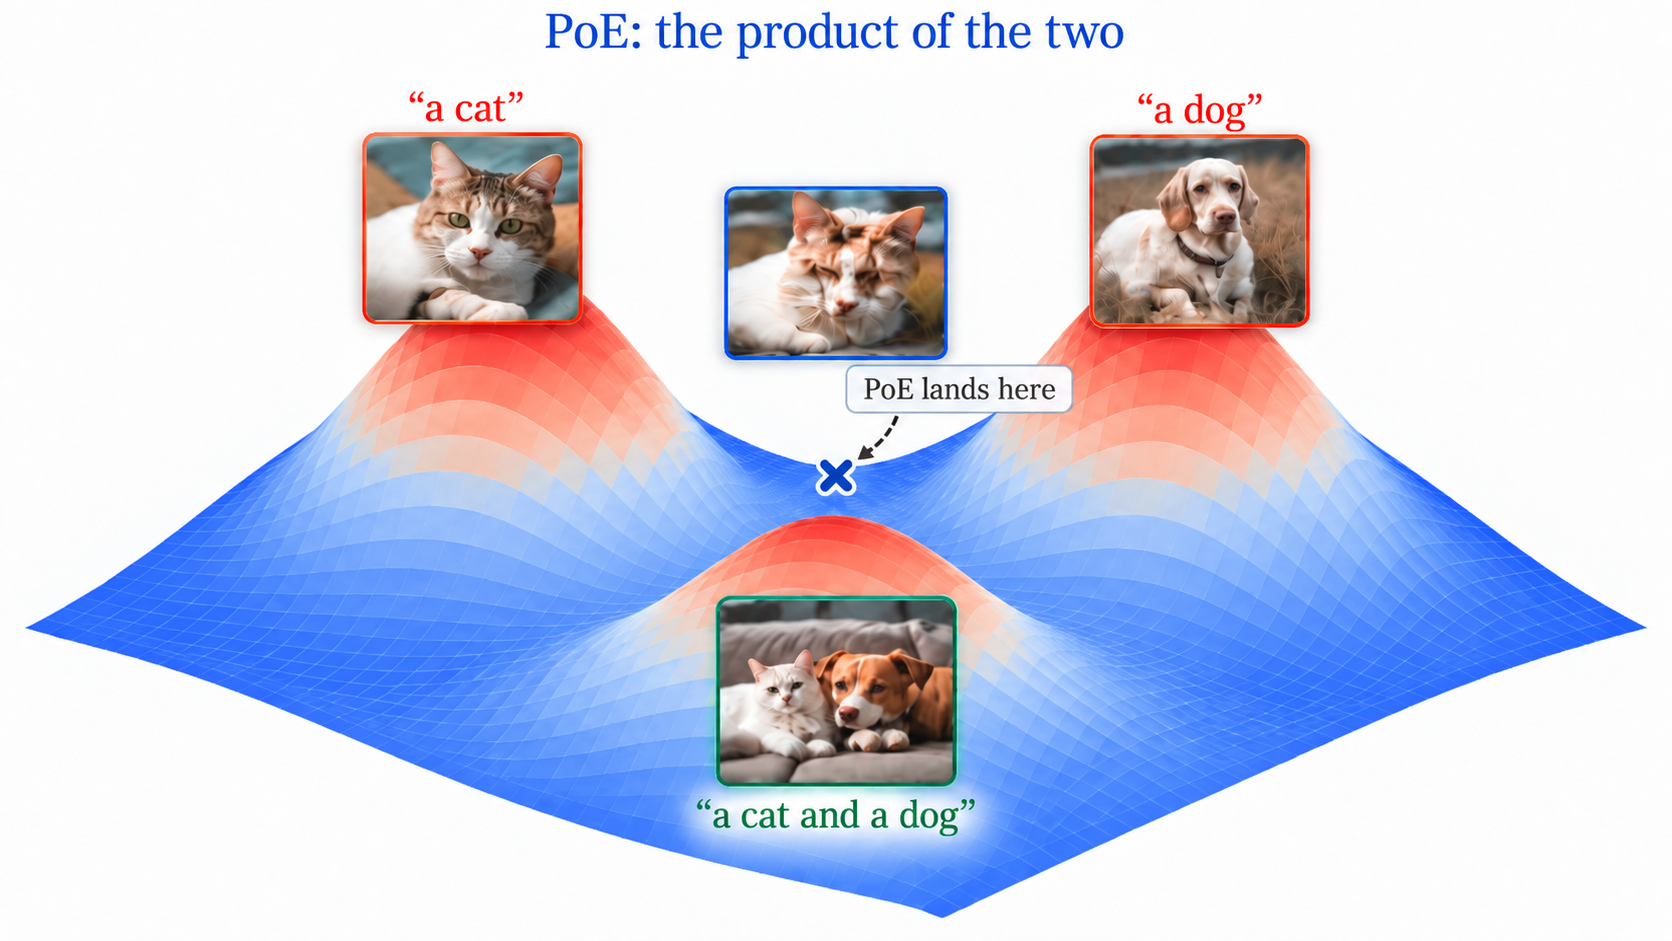
\includegraphics[width=\textwidth]{where-the-product-lands-on-the-manifold-seed12-surface.png}
\caption{\textbf{Product-of-experts composition lands between the two concepts rather than on the scene the joint prompt reaches.} All four renders are the same sampler from the same starting noise, differing only in what conditions it: the first concept alone, the second alone, both concepts composed, and the joint prompt naming the scene. Composing two concepts multiplies their distributions, which adds their scores, and the sampler follows that sum to the maximum of the product, which for two separated peaks lies between them. That maximum is the image satisfying both experts at once, and when two animals compete for the same region of the picture the only such image is a single blended animal \citep{bradley2025mechanisms}. The surface is drawn to show that geometry and is not a measured landscape; the four renders on it are real samples.}
\label{fig:poe-failure}
\end{figure}


Natural images usually depict several objects that appear together and interact as part of a coherent scene. A cat may sit beside a dog, or a cup may rest on a table, so generating such a scene takes more than producing each object correctly. The model must also place them, so a cup described as resting on a table sits on the tabletop rather than floating above it, appearing underneath it, or merging into its surface.

Recently, text-to-image diffusion models \citep{saharia2022photorealistic, podell2023sdxl} have demonstrated a remarkable ability to generate complex scenes with high visual fidelity. Much of this progress has been driven by scaling model capacity and training data, enabling these models to represent a broad range of objects and their interactions within a scene. Recent work has shown that these models can also capture aspects of the physical structure of visual scenes \citep{chen2023beyond, du2024generative}. Despite this progress, they remain unreliable on several forms of compositional reasoning, including counting \citep{huang2025t2icompbench}, negation \citep{conwell2024relations}, and attribute binding \citep{huang2025t2icompbench}. Many specific concept compositions also remain rare or unseen during training \citep{du2024compositional}, which has motivated methods that compose pretrained diffusion models directly at inference time, without additional training \citep{liu2022compositional}.

In text-to-image diffusion models, the conditioning signal $(c)$ is typically derived from a text prompt and used to guide the reverse process. Models such as Stable Diffusion \citep{rombach2022high} condition the denoising network on these text representations. For example, one model conditioned on \textit{``a cat and a dog''} handles the whole request, placing both animals in the same scene. We call this setting \textbf{joint prompting}, or \textbf{Mono}, and it is the reference the rest of this paper measures against.

We contrast this with \textbf{inference-time composition}, where the concepts are represented by separate pretrained conditional models. For example, one model may be conditioned on \textit{``a cat''} and another on \textit{``a dog''}. Their predictions are then combined during the reverse process using a product-of-experts (PoE) formulation \citep{liu2022compositional, zhang2025product} to generate a sample that satisfies both conditions. Unlike joint prompting, the composed model has not been trained directly on the joint condition. In practice, this setting often fails to preserve the constituent concepts as distinct objects. Instead, the composition can collapse into a single entangled or hybrid object. The property lost in this collapse is what we call \textbf{plurality}, the property that every concept a prompt names appears in the scene as its own distinct object. We study this gap between joint generation and inference-time composition and investigate why PoE composition fails even when the individual models represent each concept well.

% Product-of-experts composition assumes the two concepts are conditionally independent given the image \citep{bradley2025mechanisms}. Section~\ref{sec:interaction} derives what follows from that assumption, and what it leaves out.

In diffusion models, the noise prediction is a scaled negative score: $\epsilon_\theta(x_t, t \mid c) = -\sigma_t \nabla_{x_t} \log p(x_t \mid c)$ \citep{dhariwal2021diffusion}, where $\sigma_t$ is the noise standard deviation at step $t$. The assumption then gives the product-of-experts composition rule:
\begin{equation}
\hat\epsilon_{\mathrm{PoE}}(x_t,t) = \epsilon_\theta(x_t,t\mid c_1) + \epsilon_\theta(x_t,t\mid c_2) - \epsilon_\theta(x_t,t),
\label{eq:poe-composition}
\end{equation}

This linear composition is exact only when the two concepts are truly conditionally independent given the image. Natural concepts, however, interact through appearance, geometry, and spatial arrangement. The gap between what the true joint model would predict and what PoE predicts is an interaction term, the quantity a product of independent experts drops. In our setting it is narrowed to plurality, so we call it the plurality term $r_t$, and it is this missing term that we measure, understand, and learn to correct.

\looseness=-1
To make this concrete, consider two visually similar concepts: a cat and a dog. When prompted jointly, a single model trained on both concepts generates two distinct animals in one scene. When the same two concepts are composed using product-of-experts, the result is a single blended animal that combines features of both, as shown in Figure~\ref{fig:poe-failure}. This failure is not incidental; it reflects a systematic gap in how PoE composition works, one we make explicit and study throughout this paper.

Understanding and fixing this gap matters because inference-time composition is the practical path forward for generative models. As the space of possible concept combinations grows, retraining on every combination becomes infeasible \citep{du2024compositional}. Composition methods that work reliably, even for concept pairs unseen during training, unlock a new mode of model reuse: combine pretrained models without additional training, and get reliable compositional generation. This paper traces a specific failure in one composition method and shows that the failure is correctable. This paper makes three contributions:
\begin{itemize}
    \item \textbf{We define the plurality term.} We write $r_t$ as the step-by-step difference between the model's joint-prompt prediction and its PoE prediction, turning the missing compositional signal into a quantity we can measure and correct.
    \item \textbf{We show the plurality term is the signal that restores composition.} Adding the correct residual turns PoE failures into two-object scenes; mismatched residuals of comparable size do not have this effect.
    \item \textbf{We learn a lightweight correction that transfers.} A low-rank adapter on SDXL's cross-attention layers predicts $r_t$ without access to the joint prompt and composes concept pairs excluded from its training set.
\end{itemize}

\section{Background and Related Work}
\label{sec:background}

Recent methods compose pretrained diffusion models at inference by sampling from the product of the individual concept distributions. Conditioning a pretrained model on a single concept prompt concentrates its distribution on images showing that concept, and this conditional distribution is each expert's contribution to the product. This multiplication is the product-of-experts construction \citep{liu2022compositional, zhang2025product}, in which the product stays large only on images to which every expert assigns high probability, so a sample must satisfy both concepts at once. A prompt such as ``a cat and a dog'' asks for plurality, each concept appearing in the scene as its own distinct object, the way the two animals co-occur in captioned training images. Assigning high probability under both experts and appearing as two distinct objects in one scene are different demands, and the product enforces only the first. In this paper we focus on conflicting concept pairs, where composition loses plurality, and show that the loss is measurable as a per-step residual that can be learned.

Existing methods keep the product as the target and improve how it is composed and sampled \citep{dutta2026steer, huang2026factordiff, wang2026testtime}. \citet{liu2022compositional} treat a prompt naming two concepts as a conjunction, one expert per concept, and add the experts' predictions directly at each denoising step. \citet{du2023reduce} show that reverse diffusion on the composed predictions does not sample the product the addition aims at, and correct the mismatch with Markov chain sampling. Later methods sharpen the correction, with annealed importance sampling \citep{zhang2025product} and sequential Monte Carlo correctors \citep{skreta2024superdiff, skreta2025feynman}. The rest of this section lays out how the predictions these methods combine are produced, and where the assumption of independence between the composed concepts enters.

\paragraph{Diffusion models.} A diffusion model generates an image by starting from pure Gaussian noise and removing noise step by step. A fixed process turns an image $x_0$ into pure noise $x_T$, adding Gaussian noise one step at a time to produce the intermediate versions $x_1, \dots, x_{T-1}$ \citep{sohldickstein2015deep, ho2020denoising}. Since each step's noise is independent and Gaussian, the whole chain from $x_0$ to any $x_t$ collapses into one jump,
\begin{equation}
x_t = \sqrt{\bar\alpha_t}\, x_0 + \sqrt{1-\bar\alpha_t}\,\epsilon, \qquad \epsilon \sim \mathcal{N}(0, I),
\label{eq:forward}
\end{equation}
with $\bar\alpha_t = \prod_{s\le t}\alpha_s$ the accumulated product of the per-step noise levels. A network $\epsilon_\theta(x_t, t \mid c)$ is trained to predict which noise $\epsilon$ was added at step $t$, given the noised latent $x_t$ and a conditioning prompt $c$,
\begin{equation}
\mathcal{L} = \mathbb{E}\,\lVert \epsilon - \epsilon_\theta(x_t, t \mid c) \rVert^2.
\label{eq:objective}
\end{equation}

\paragraph{Noise predictions are scores.} A network that predicts the added noise is also estimating the score of the noised data distribution, the gradient of its log density \citep{song2021scorebased}. The noise prediction is the score scaled by the noise level,
\begin{equation}
\epsilon_\theta(x_t, t \mid c) = -\sigma_t\, \nabla_{x_t} \log p_\theta(x_t \mid c),
\label{eq:score}
\end{equation}
where $\sigma_t = \sqrt{1-\bar\alpha_t}$ \citep{dhariwal2021diffusion}.

\paragraph{Classifier-free guidance.} Classifier-free guidance trains a single network as both a conditional and an unconditional model, by replacing the prompt with a null token on a fraction of the training steps, and at every sampling step combines the two predictions it produces \citep{ho2022classifier},
\begin{equation}
\hat\epsilon(x_t, t \mid c) = \epsilon_\theta(x_t, t) + w\,\big[\,\epsilon_\theta(x_t, t \mid c) - \epsilon_\theta(x_t, t)\,\big].
\label{eq:cfg}
\end{equation}
Raising $w$ trades sample diversity for fidelity to the prompt. The composition rule in \eqref{eq:poe-composition} combines one conditional prediction per concept with the same unconditional one.

The combination in \eqref{eq:poe-composition} samples from a composition of the concepts' conditional marginals under the assumption that the concepts are statistically independent given the image. \citet{bradley2025mechanisms} study when linear score combination provably achieves the intended composition, whether reverse-diffusion sampling can then generate it, and the conditions under which it fails. \citet{gaudi2025coind} show that standard conditional diffusion models violate the independence assumption even when every attribute composition is observed in training, more severely when only a subset is, and enforce the assumption during training by minimising the Fisher divergence between the model's joint conditional and the product of its single-concept conditionals. The next section measures what that failure removes from a pretrained model.

\section{Missing Implications: The Plurality Term}
\label{sec:interaction}

At each denoising step, product-of-experts composition evaluates the pretrained network on the same latent $x_t$ under three conditions, the first prompt, the second prompt, and no prompt at all. With no prompt, the network's prediction moves the latent toward images in general rather than toward either concept. These three predictions are then combined to form the PoE noise estimate given in \eqref{eq:poe-composition}, by adding the two conditional predictions and subtracting the unconditional one. Each conditional prediction contains the unconditional prediction plus a term carrying its own prompt. Three properties of this construction carry into the rest of the section: nothing is trained, the network is never shown both prompts at once, and the composed prediction is a fixed linear combination of three of its own outputs.

When the two concepts are independent given the image, the joint density factorises as $p(x \mid c_1, c_2) \propto p(x \mid c_1)\, p(x \mid c_2)\,/\,p(x)$ \citep{liu2022compositional}. The unconditional density is in the denominator because it is already contained in both conditional experts, so their product carries it twice and one copy has to be removed. Taking logarithms and passing to noise predictions gives the estimate the sampler uses, writing $p_{\mathrm{PoE}}$ for the product above.
\begin{align}
\log p_{\mathrm{PoE}}
  &= \log p(x \mid c_1) + \log p(x \mid c_2) - \log p(x) + \text{const} \\
\nabla_x \log p_{\mathrm{PoE}}
  &= \nabla_x \log p(x \mid c_1) + \nabla_x \log p(x \mid c_2) - \nabla_x \log p(x) \\
\hat\epsilon_{\mathrm{PoE}}(x_t, t)
  &= \epsilon_\theta(x_t, t \mid c_1) + \epsilon_\theta(x_t, t \mid c_2) - \epsilon_\theta(x_t, t) \\
  &= \epsilon_\theta(x_t, t) + \sum_{i=1}^{2}
     \big[ \epsilon_\theta(x_t, t \mid c_i) - \epsilon_\theta(x_t, t) \big]
\end{align}

Attaching a weight $w_i$ to each conditional term gives $\hat\epsilon = \epsilon_\theta(x_t,t) + \sum_i w_i[\epsilon_\theta(x_t,t \mid c_i) - \epsilon_\theta(x_t,t)]$, which is the form used in practice \citep[equation 11]{liu2022compositional} and which recovers the derivation exactly at $w_i = 1$.

The gap between the joint conditional and the product form is the ratio $R_t = p(c_1, c_2 \mid x_t)\,/\,\big(p(c_1 \mid x_t)\, p(c_2 \mid x_t)\big)$. $R_t$ equals one exactly when the two concepts are independent given the state. Keeping this ratio instead of setting it to one turns the product form back into the joint, $p(x_t \mid c_1, c_2) \propto p_{\mathrm{PoE}}(x_t \mid c_1, c_2)\, R_t$.

At every step the sampler combines the two experts as though this factor were one, whether or not it is. Which images the product favours depends on where the two experts overlap, and for two subjects contending for one region it peaks between them rather than on an image holding both \citep{bradley2025mechanisms, dutta2026steer}. Writing $\epsilon_{\text{true}}$ for the noise prediction of the true joint score, which no model gives us,
\begin{align}
\nabla_{x_t} \log p(x_t \mid c_1, c_2)
  &= \nabla_{x_t} \log p_{\mathrm{PoE}}(x_t \mid c_1, c_2) + \nabla_{x_t} \log R_t \\
-\sigma_t \nabla_{x_t} \log p(x_t \mid c_1, c_2)
  &= -\sigma_t \nabla_{x_t} \log p_{\mathrm{PoE}}(x_t \mid c_1, c_2) - \sigma_t \nabla_{x_t} \log R_t \\
\epsilon_{\text{true}}(x_t, t)
  &= \hat\epsilon_{\mathrm{PoE}}(x_t, t) - \sigma_t \nabla_{x_t} \log R_t
\end{align}

Nothing in the run evaluates $R_t$, so the paper measures the gap between the two predictions the network does produce instead. The same rule composes one pair and blends another (Figure~\ref{fig:two-regimes}), so whatever separates the two cases is not the rule itself. $R_t$ is a property of the two concepts and $r_t$ is a property of one model's two predictions, so no reading of size carries from one to the other, and two pairs cannot say whether the size of the correction predicts which pairs fail. When the correction has to arrive is what we measure next.

\begin{figure}[!tb]
\centering
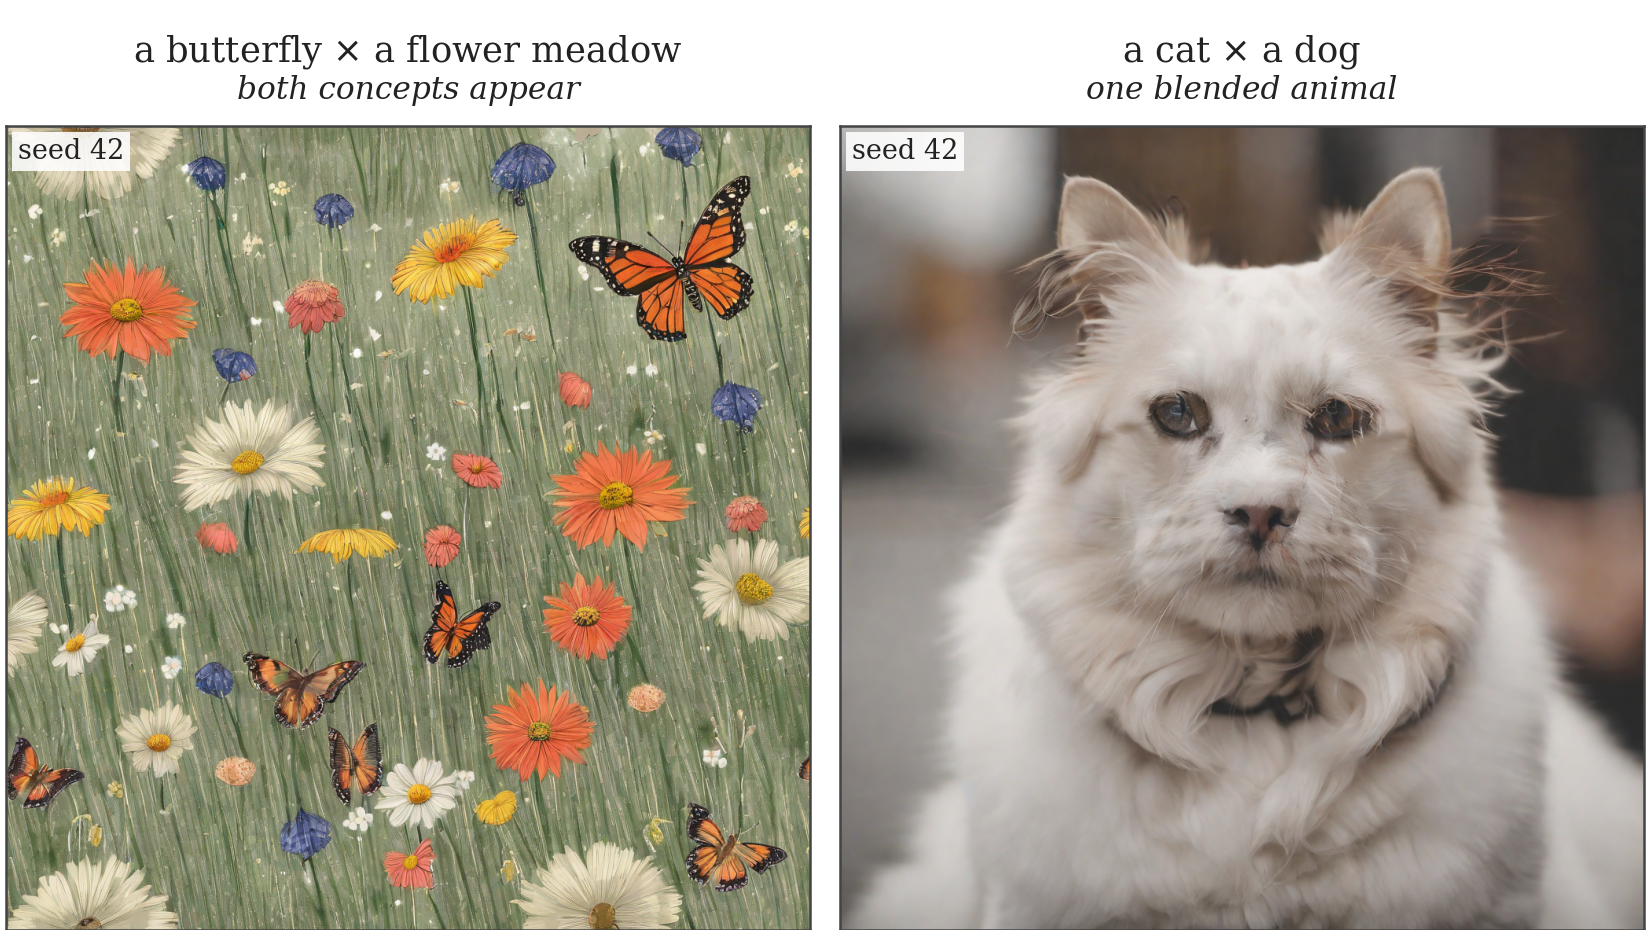
\includegraphics[width=0.62\textwidth]{same-rule-composes-one-pair-and-blends-another.pdf}
\caption{\textbf{The same rule composes one pair and blends another.} One real sample per prompt pair, seed 42, both sampled with uncorrected product-of-experts composition at the same settings. The butterfly pair puts both concepts in the picture; the animal pair returns one blended animal.}
\label{fig:two-regimes}
\end{figure}

We define the plurality term $r_t$ as the difference between the model's prediction under the joint prompt, written $\epsilon_{\mathrm{Mono}}$, and its product-of-experts prediction, both evaluated on the same latent $x_t$.
\begin{equation}
r_t \;=\; \epsilon_{\mathrm{Mono}}(x_t, t) \;-\; \hat\epsilon_{\mathrm{PoE}}(x_t, t)
\label{eq:interaction-term}
\end{equation}

The identity $\epsilon_{\mathrm{Mono}} = \hat\epsilon_{\mathrm{PoE}} + r_t$ holds by construction and is not a result, whereas the size of $r_t$, its structure across denoising steps, and its transfer to concept pairs held out of training are. Correcting the sampler means adding a scaled copy of $r_t$ back at each step, with $\lambda = 0$ leaving composition uncorrected and $\lambda = 1$ reproducing the joint-prompt prediction exactly.
\begin{equation}
\hat\epsilon_\lambda(x_t, t) = \hat\epsilon_{\mathrm{PoE}}(x_t, t) + \lambda\, r_t
\label{eq:corrected-sampler}
\end{equation}

\looseness=-1
The strength axis separates the correction from any disturbance of the same size and schedule. In Figure~\ref{fig:strength-grid} the fusion holds until $\lambda$ reaches 0.75 and then resolves into a cat and a dog, while no control reaches two animals at any strength, so what restores composition is where the correction points rather than how hard the prediction is disturbed. The rows part company hardest past $\lambda = 1$, where the measured correction still gives two clean animals at $\lambda = 2$ and every control has collapsed into colour artefacts or a single chimera. One pair at one seed illustrates the strength axis rather than measuring it.

\begin{figure}[!b]
\centering
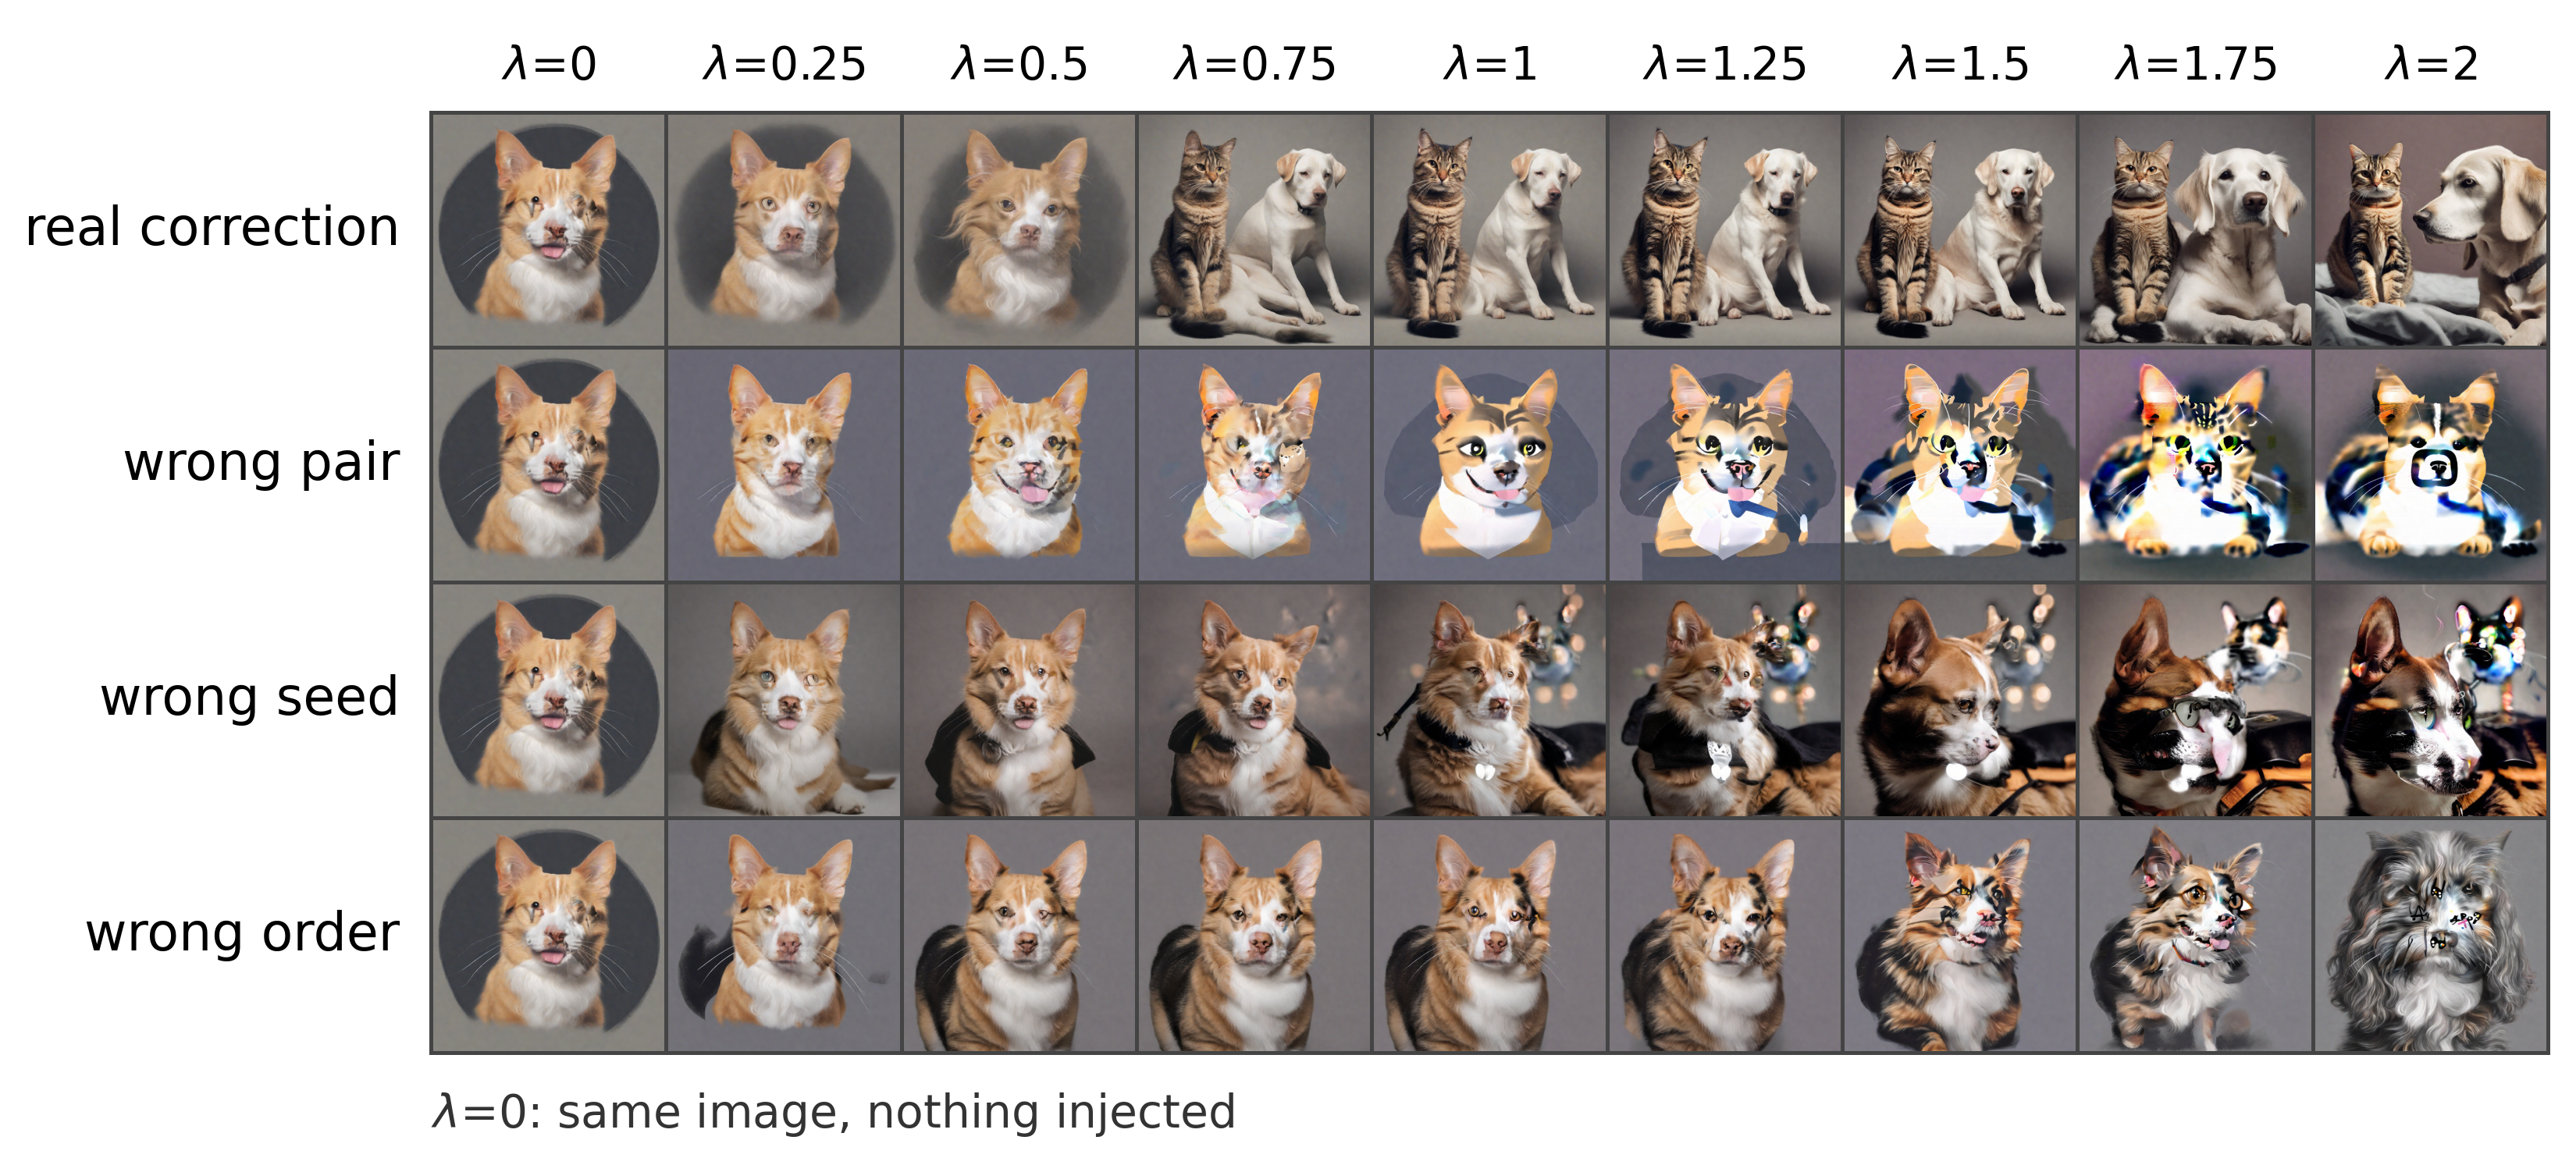
\includegraphics[width=\textwidth]{how-much-is-added/strength-grid.pdf}
\caption{\textbf{Only the measured correction composes, and over-driving it does no visible harm.}
A cat and a dog at seed 9. A column is the strength $\lambda$ added at every step; a row is what was
added. The top row is the pair's own plurality term, and beneath it sit three controls, each breaking
one thing about it while matching its size and schedule: another pair's term, the same term from a
different seed, and the same term with its step order deranged. Nothing is added at $\lambda = 0$, so
that column is one sample shown four times, and the columns past $\lambda = 1$ carry the correction
beyond the joint-prompt prediction.}
\label{fig:strength-grid}
\end{figure}

Product-of-experts sampling never sees the joint prompt. The difference $r_t$ therefore serves as a signal we can measure, one that establishes what the missing correction is, when in the denoising trajectory it matters, and why composition fails without it. $r_t$ is a full noise-prediction vector at every step, so it has a direction as well as a magnitude.

Independence can fail in more than one way, and the one this paper studies is spatial, since a patch of pixels that reads strongly as one animal cannot read equally strongly as the other. In every pair we study both concepts are foreground subjects, rather than a subject and a setting that could occupy different parts of the image. The same network produces two distinct animals when it is given the joint prompt, so the failure belongs to the composition rule and not to the model.

The composed prediction and the joint prediction are built from the same four conditional evaluations at every denoising step: the first concept, the second, the joint prompt, and no prompt. Both are read at the same latent $x_t$, the one the corrected sampler is currently visiting, so $r_t$ is measured along the trajectory it is applied to rather than imported from a separate run. The true joint score $\nabla_x \log p(x \mid c_1, c_2)$ is a property of the world, whereas $\epsilon_{\mathrm{Mono}}$ is what this network outputs when its text encoder is handed one prompt naming both concepts. So $r_t$ measures a gap between two behaviours of one model, not a gap to the correct distribution. Every term in $r_t$ is one network's own output at the state the sampler has reached, so the missing piece can be measured on any run without knowing the true joint distribution. Restoring it can therefore only recover what joint prompting already does, which is the behaviour inference-time composition is trying to reproduce.

\section{Restoring the Plurality Term Restores Composition}
\label{sec:analysis}

If $r_t$ is the signal composition is missing, then adding back a fraction $\lambda$ of it should compose the pair, and both $\lambda$ and which steps receive it should matter. We show that a small fraction of the measured plurality term, applied in the first steps of the denoising run, is enough to restore composition. The strength axis says nothing about when the correction has to be present. A composed run visits fifty states and the correction is defined at every one of them, so restoring composition could need the whole trajectory or only part of it. The difference decides what a learned correction has to do: a term needed everywhere must be produced at every step of every run, while a term needed only at the start has to be right in a narrow window and can leave the rest to plain composition. We settle it by choosing which steps receive the correction and leaving the others uncorrected.

One pair shows what the sweep that follows measures across every pair. Extending the correction later into the run buys nothing, and starting it later than step ten loses composition altogether (Figure~\ref{fig:when-the-correction-arrives}). Both grids are one pair at one seed, so nothing here says how often that boundary holds.

\begin{figure}[!ht]
\centering
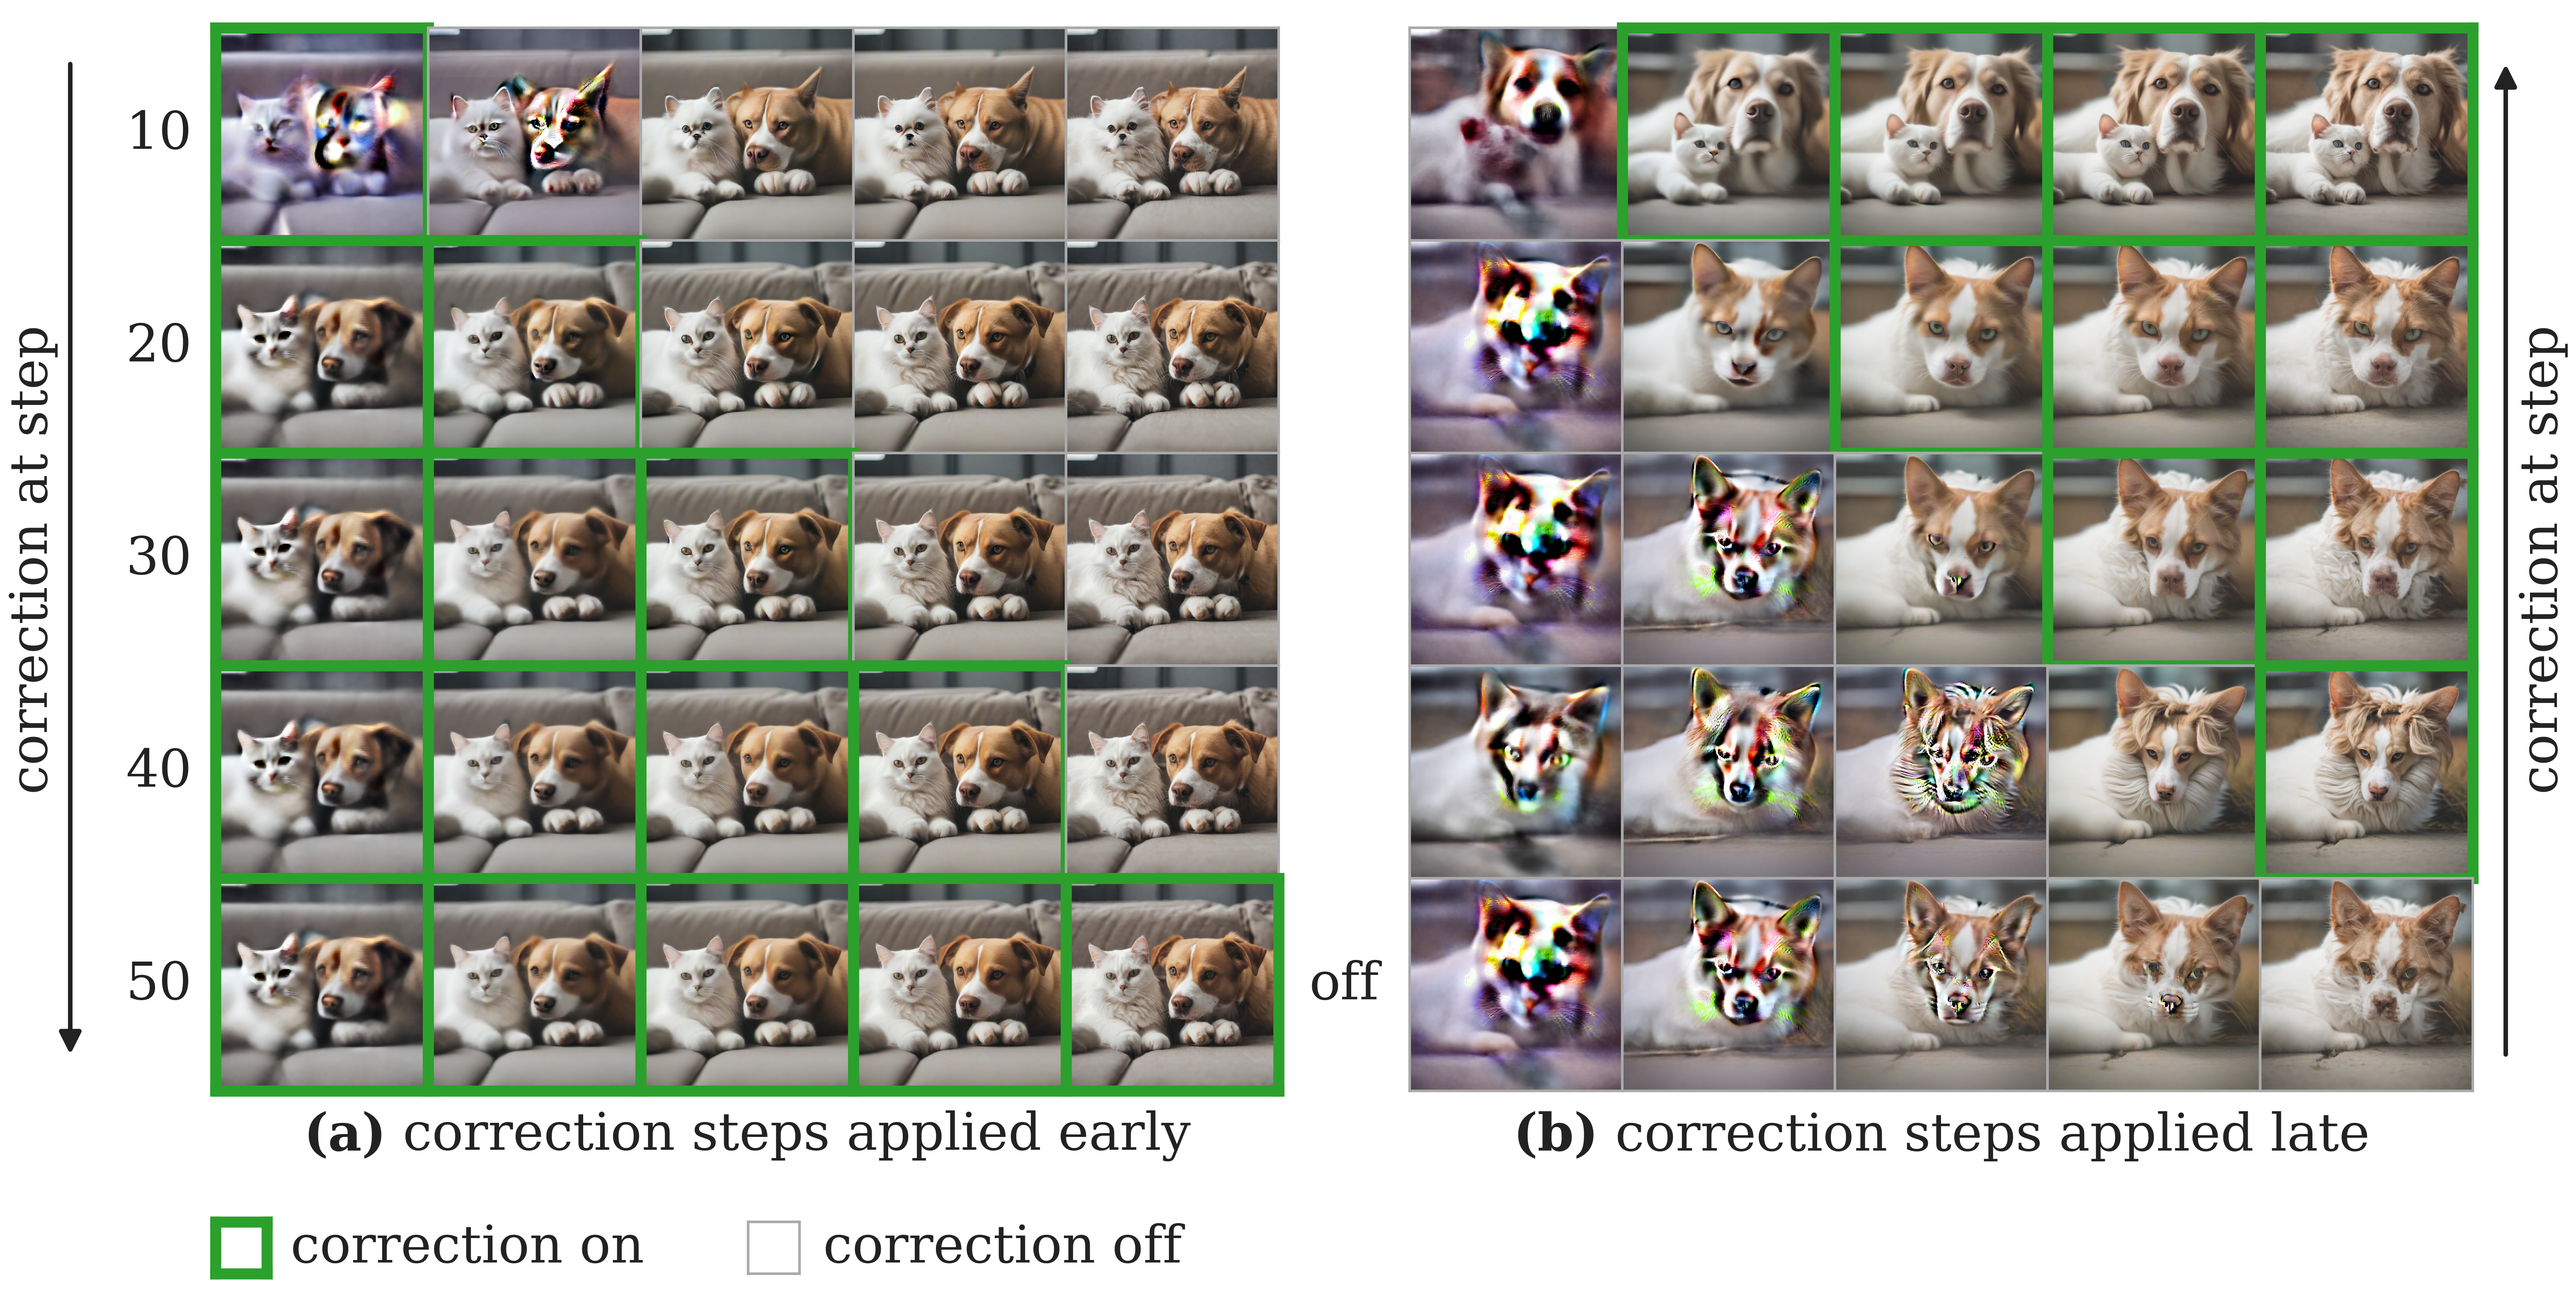
\includegraphics[width=\textwidth]{when-the-correction-arrives/when-the-correction-arrives.pdf}
\caption{\textbf{Ten corrected steps already reach the outcome, and no late start recovers it.}
A cat and a dog at seed 12. Two grids of the same run, differing only in which stretch of it receives
the correction: from the beginning outward in \textbf{(a)}, from a later start through to the end in
\textbf{(b)}. Along any row the five pictures are that run decoded after 10, 20, 30, 40 and 50 steps,
a green frame marks a decode taken while the correction was active, and the row marked \emph{off}
never corrects. Read down the rightmost column of each panel: in (a) it never changes, and in (b) it
changes exactly once, between the row that starts at step ten and the row that starts at step twenty.}
\label{fig:when-the-correction-arrives}
\end{figure}


% Commented out while the timing argument is carried by fig:where-the-correction-lands alone.
% \begin{figure}[!tb]
% \centering
% 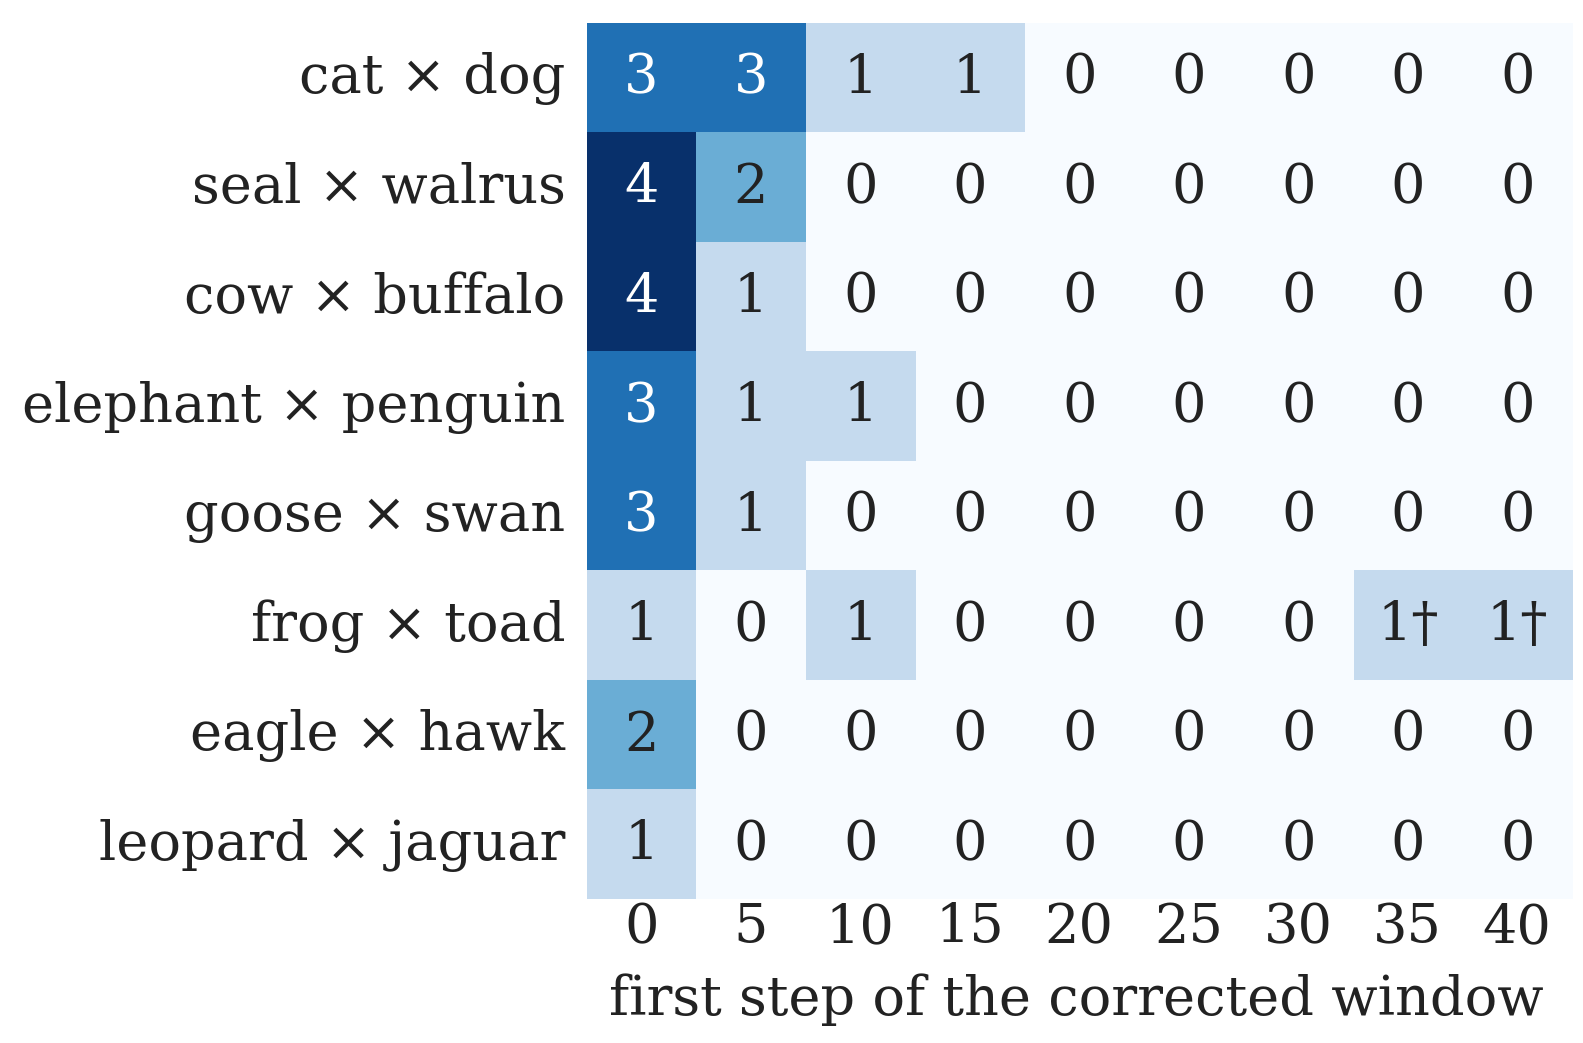
\includegraphics[width=0.62\textwidth]{how-often-the-correction-lands.pdf}
% \caption{\textbf{Only windows that start in the first steps restore composition, and the boundary
% falls in the same place for every pair.} Seeds composed, of four, for every pair as the ten-step
% correction window slides across the run. Daggers mark detector error, a single animal boxed twice.}
% \label{fig:how-often-the-correction-lands}
% \end{figure}

The sweep across all eight pairs and four seeds draws the same boundary. A generated image counts as composed when an object detector finds two distinct animals in it, and all counts were manually verified. We restrict the correction to a ten-step window, leave the remaining forty steps uncorrected, and slide the window across the run in strides of five. The window is kept narrow so the sweep can separate timing from coverage, since a window spanning most of the run would contain the early steps at every position. Windows starting within the first five steps restore composition for every pair we tried, and windows starting at step 20 or later restore it for none (Figure~\ref{fig:where-the-correction-lands}). The correction is therefore not needed for most of the run: once the early steps have settled which scene the trajectory is in, plain product-of-experts composition carries the image to the end without it. In every pair we measured, the correction is at its smallest, relative to that pair's typical per-step size, in the steps where it matters, so size does not explain the timing. Why the earliest steps are decisive is open, and what we can show is that the correction they need is learnable. Every result above used the joint prompt, which composition is not allowed to have. The next section removes that need.

\begin{figure}[!ht]
\centering
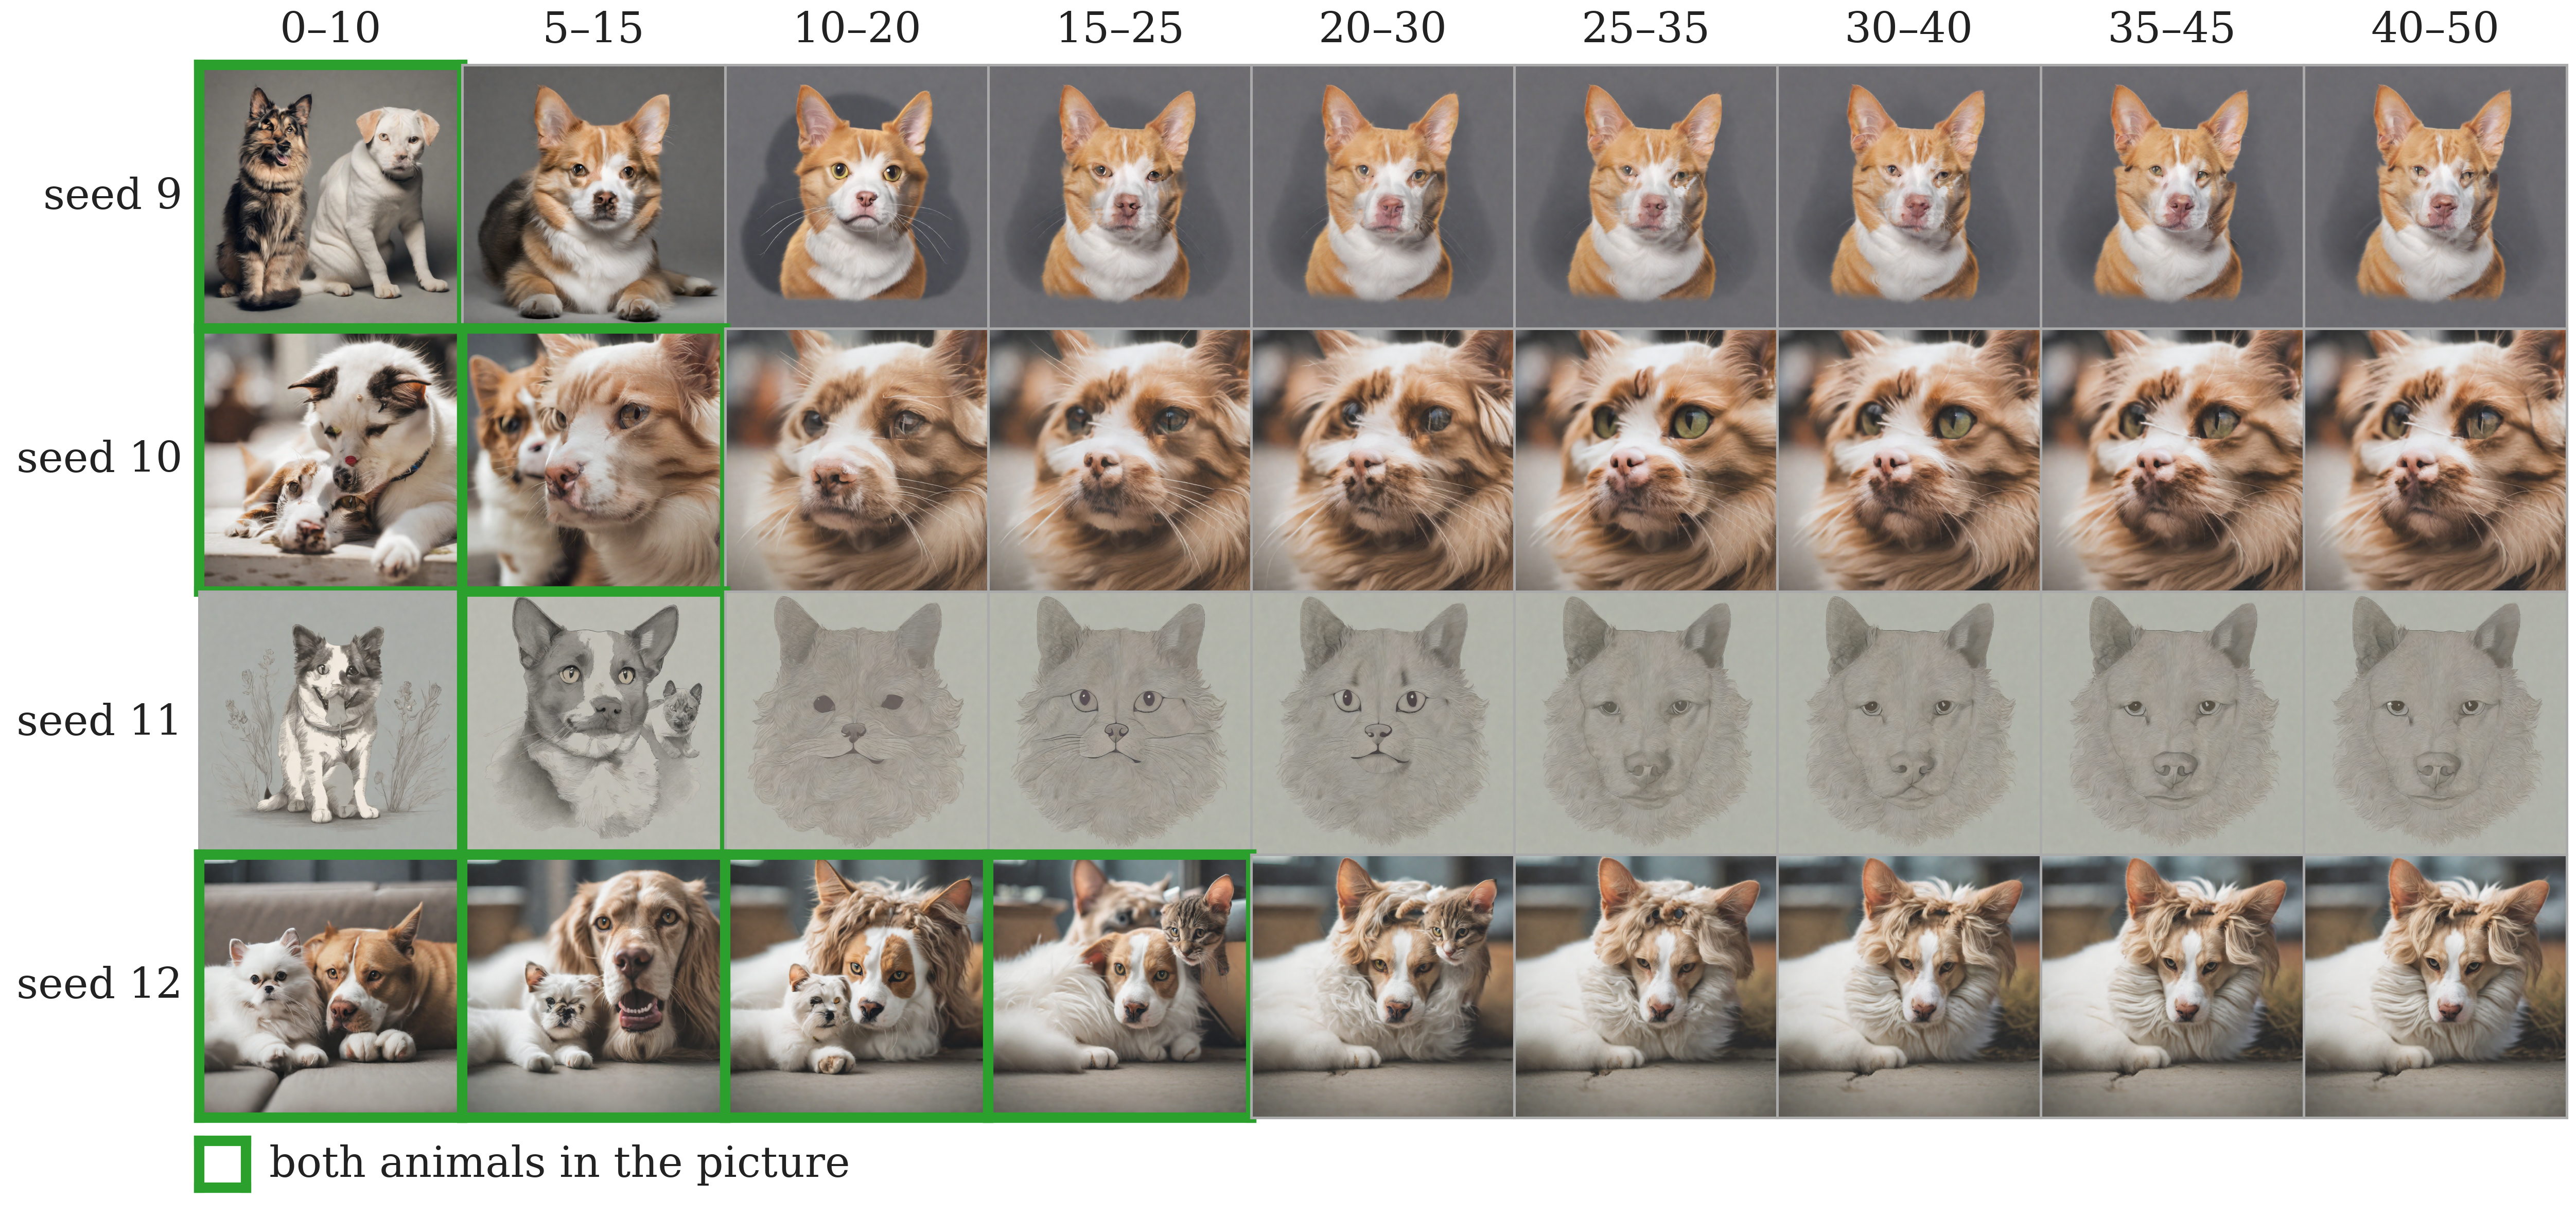
\includegraphics[width=\textwidth]{where-the-correction-lands.pdf}
\caption{The final image for a cat and a dog at seeds 9 to 12, as the ten-step correction window
slides across the run. A column is the window's first and last step, and everything outside it runs
plain composition, so a row varies only in where the correction sat. The green frame is the
detector verdict, a cat box and a dog box with little overlap. Seed 11
composes at 5--15 but not at 0--10, the one break in the left-to-right decay.}
\label{fig:where-the-correction-lands}
\end{figure}


\section{Learning the Plurality Term}
\label{sec:method}
\looseness=-1
In the previous section we measured the plurality term along composed runs and showed that adding a small amount of it back, early in the run, restores composition. In this section we learn it. We train a model that produces the correction at each step, from the current state and the two concept prompts, so a corrected run no longer needs the joint prompt. The joint prompt is barred only at inference, so the term can still be measured in advance, and those measurements are what the model trains on.

The model learns its correction from the residuals themselves. For each training pair we therefore store the residual at every denoising step, over several runs, so the training data covers whole trajectories rather than isolated steps. We train a single adapter on every pair together to learn the correction rule that restores the plurality lost during composition.

The adapter is a low-rank adaptation (LoRA) of rank 8 on the query, key and value projections of every cross-attention layer, with the base model frozen. At each step of the run the UNet takes two inputs, the current latent $x_t$ and the prompt. They meet in the cross-attention layers, where the layer projects the image to queries and the prompt's token embeddings to keys and values, so each region of the image can draw on the tokens it matches. The adapter leaves these three projection matrices untouched and adds a small trainable update beside each one, the product of two rank-8 matrices whose output is summed with the original projection's. Training moves only these added matrices, so what the adapter can change is how image regions query the prompt and what the prompt's tokens give back (Figure~\ref{fig:adapter-training}, bottom).

We split a pool of nineteen animal pairs into eleven for training and eight for evaluation. To prevent a held-out gain from coming from an animal the adapter has already seen, and to attribute it to the correction rule instead, no animal appears in more than one pair anywhere in the pool. For each training pair we then run the composed sampler from eight starting noises and, at every step, evaluate the model under the joint prompt and under the two concept prompts at the state the run has reached. The difference between the joint-prompt and composed predictions is stored as that step's residual, giving 4,400 residuals across the 88 runs. The adapter is trained so that its composed prediction matches the stored joint-prompt prediction at each state, which is the same as supplying the residual without being given the joint prompt (Figure~\ref{fig:adapter-training}, top). Collection runs use guidance scale 7.5 and 50 DDIM steps at $1024\times1024$ in fp16. Training runs for 2,000 epochs of 50 optimizer steps, 100,000 in all, with AdamW at learning rate 1e-4 and gradient clipping at 1.0. On a single NVIDIA RTX PRO 6000 this takes about seven hours and peaks at 23\,GB of memory.

\begin{figure}[!t]
\centering
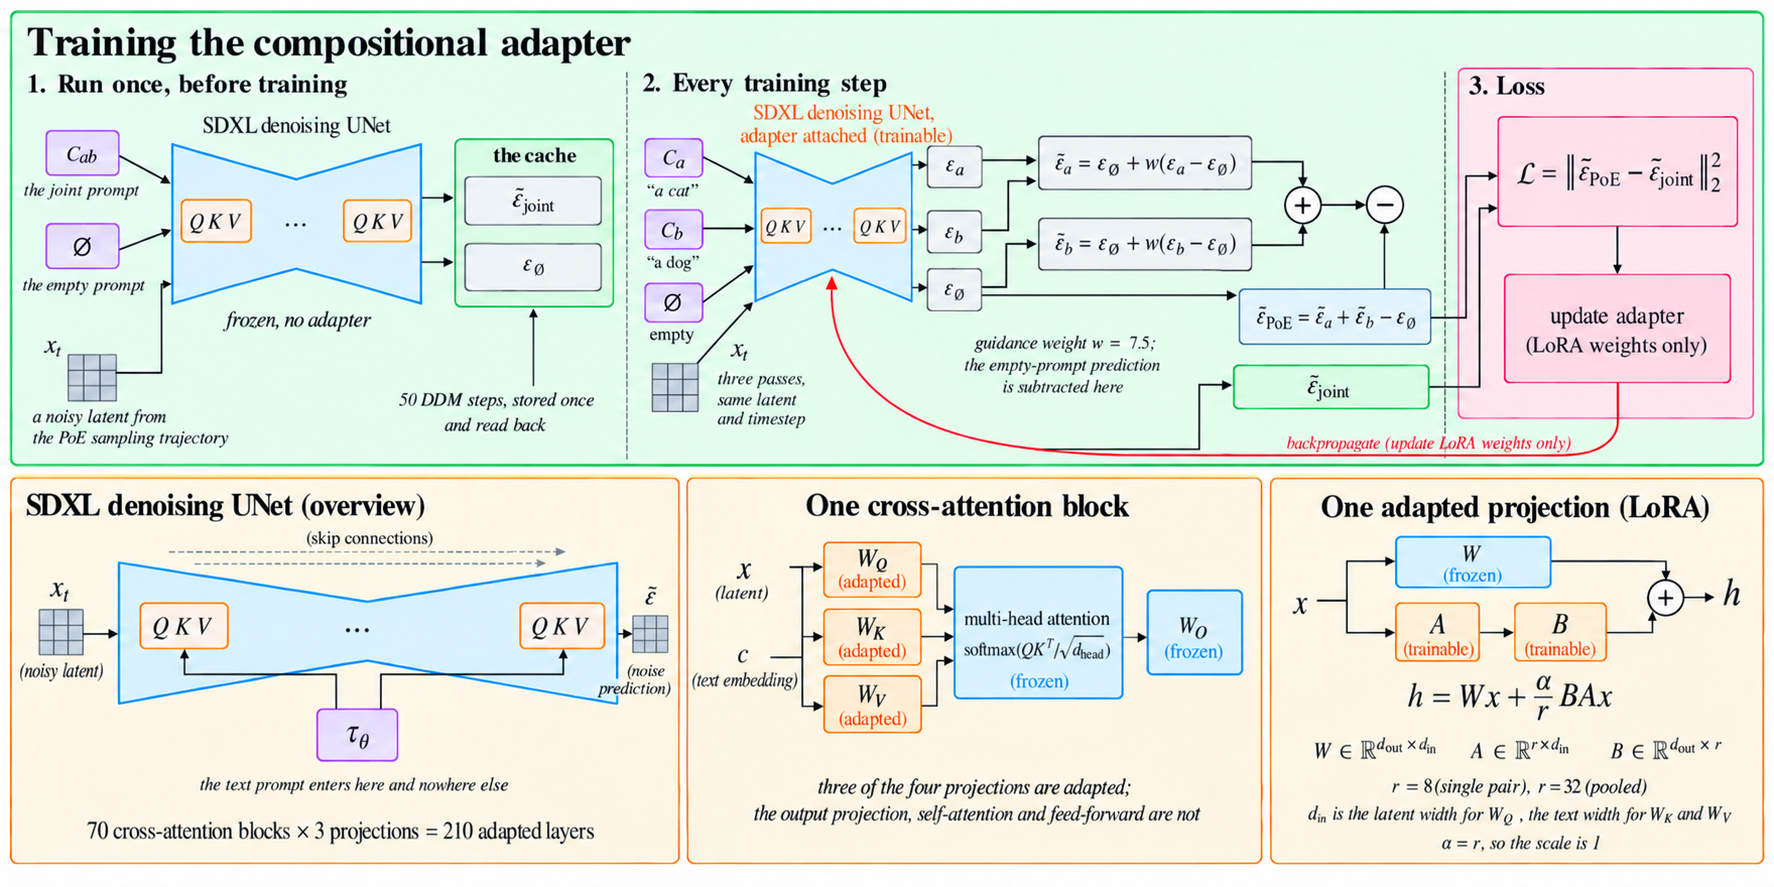
\includegraphics[width=\textwidth]{training-the-compositional-adapter.png}
\caption{\textbf{Training the compositional adapter.} \textbf{Top:} the joint-prompt prediction
$\tilde\varepsilon_{\mathrm{joint}}$ and the empty-prompt prediction $\varepsilon_{\emptyset}$ are
computed once on the frozen model along a composed run and stored. At every training step the two
concept prompts and the empty prompt are run through the adapted model at the same latent and
timestep, guided at $w = 7.5$ and combined by the product-of-experts rule, and the loss is the
squared distance between that composed prediction and the stored joint-prompt prediction. Gradients
reach the adapter and nothing else. \textbf{Bottom:} where the adapter sits. The prompt enters the
UNet only through cross-attention, and the adapter is a rank-$r$ update on the query, key and value
projections of all 70 cross-attention blocks, 210 adapted layers in total. The output projection,
the self-attention and the feed-forward layers are untouched.}
\label{fig:adapter-training}
\end{figure}

At inference the correction is not injected at all. We simply run plain product-of-experts sampling through the adapted model, with the two concept prompts and the null token as the only conditions, so the corrected sampler costs no more than the composition it repairs (Figure~\ref{fig:adapter-sampling}). Training placed the correction inside the adapter's weights, so the composition of the adapted predictions lands where the frozen model's joint-prompt prediction would have landed. For the experiments we also run each step through the frozen model, and the difference between the two composed predictions makes the learned correction explicit. Scaling that difference by $\lambda$ before stepping gives a dial on the correction, with $\lambda = 0$ recovering plain composition as a baseline and $\lambda = 1$ identical to the adapted pass alone.

\begin{figure}[!t]
\centering
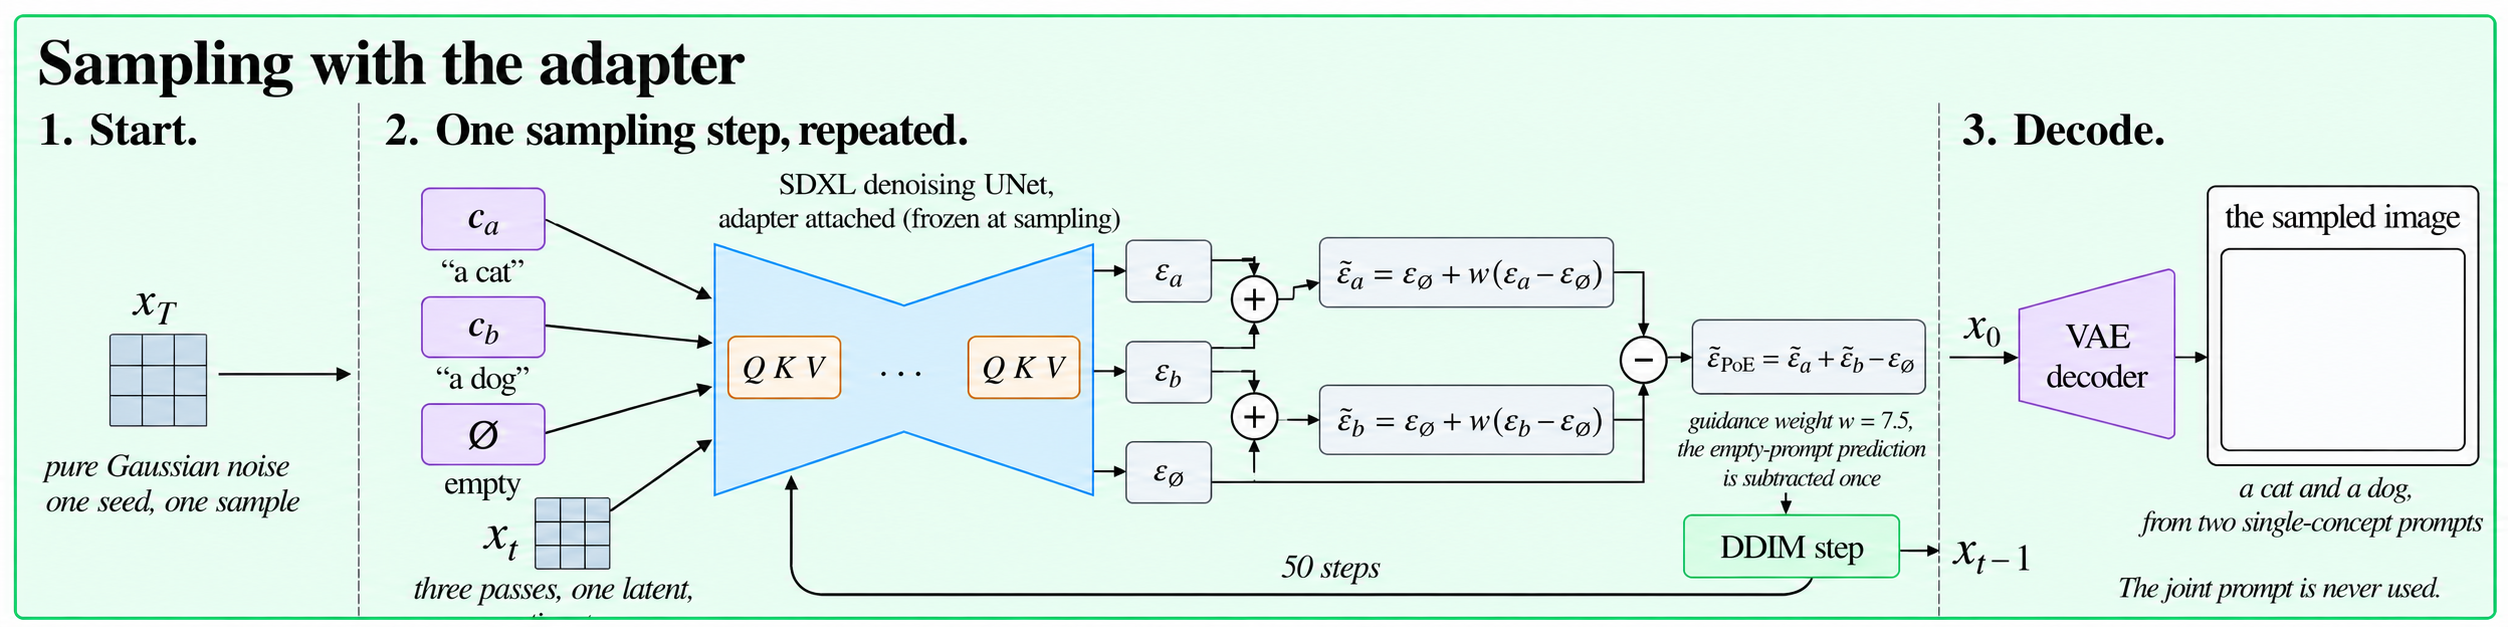
\includegraphics[width=\textwidth]{sampling-with-the-adapter.png}
\caption{\textbf{Sampling with the adapter.} One corrected run, from one starting noise. At each of
the 50 DDIM steps the current latent passes three times through the adapted model, once for each
concept prompt and once for the empty prompt. Each concept prediction is guided at $w = 7.5$ against
the empty-prompt prediction, the two are added, the empty-prompt prediction is subtracted once, and
the result takes the step. The joint prompt is never used, so the corrected sampler costs what plain
product-of-experts composition costs.}
\label{fig:adapter-sampling}
\end{figure}

On pairs the adapter never trained on, its corrected sampler reproduces what the measured correction did in the previous section, and it does so from the two concept prompts alone (Figure~\ref{fig:adapter-samples}). The correction rule therefore transfers across pairs rather than being memorised per pair, which is what the compose rate below counts.

% \begin{figure}[!htbp]
% \centering
% 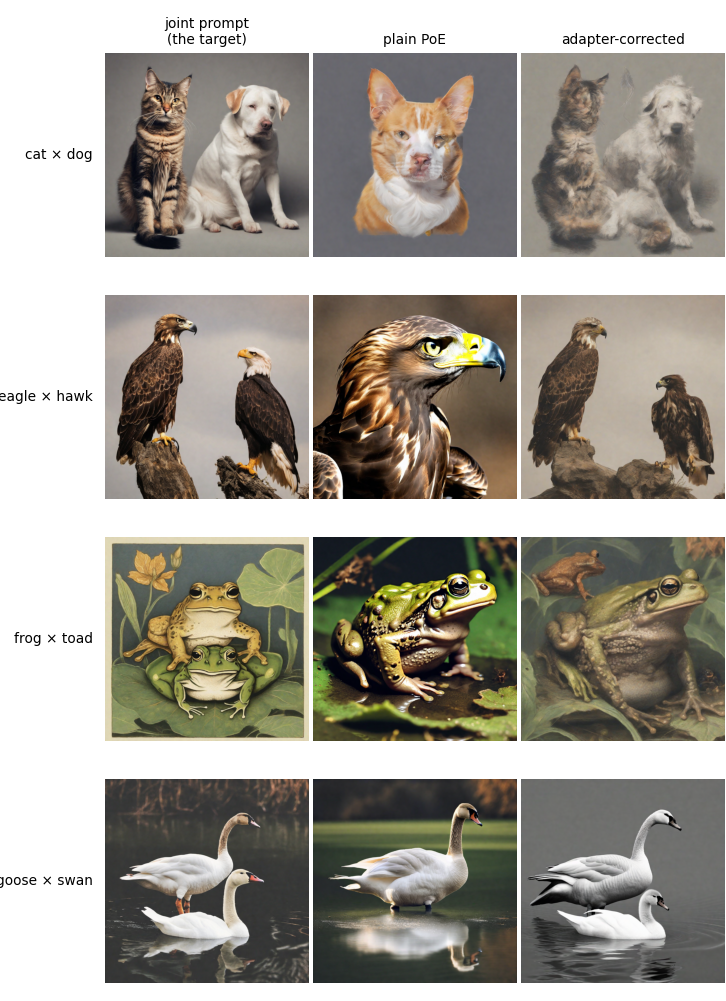
\includegraphics[width=0.5\linewidth]{joint-prompt-poe-and-adapter-samples-for-four-held-out-pairs.pdf}
% \caption{\textbf{The adapter returns held-out pairs to two animals without ever seeing the joint prompt.} Samples for four animal pairs held out of the adapter's training, under the joint prompt (left), plain product-of-experts composition (middle, one blended animal per row), and the adapter-corrected sampler (right, two distinct animals per row). The three images of a row start from the same noise, and the adapter column is the pooled checkpoint at training step 100000 with $\lambda=1$. The joint-prompt column is the target the correction was defined from, not a competing method. Four pairs illustrate the effect and do not carry the rate.}
% \label{fig:adapter-samples}
% \end{figure}

\FloatBarrier
\section{Discussion}
\label{sec:discussion}
\looseness=-1
Composition does not fail because the words attend to the wrong regions of the image. A token's key determines which regions of the latent attend to it, and its value determines what those regions receive. For every token we record both at matched states of the same run, its attention over the latent and the content written into the regions it attends to, and compare each against plain composition. The attention maps stay close to where they already were, and the content written into those regions is what moves. The same happens on an elephant and a penguin, a pair we included as a control because it is not one the product fails on. So the correction acts on what the words write, not on where they look, and that holds wherever the update is applied, which locates the correction without explaining why it repairs the pairs that fail.

\begin{wrapfigure}[40]{r}{0.5\linewidth}
    \centering
    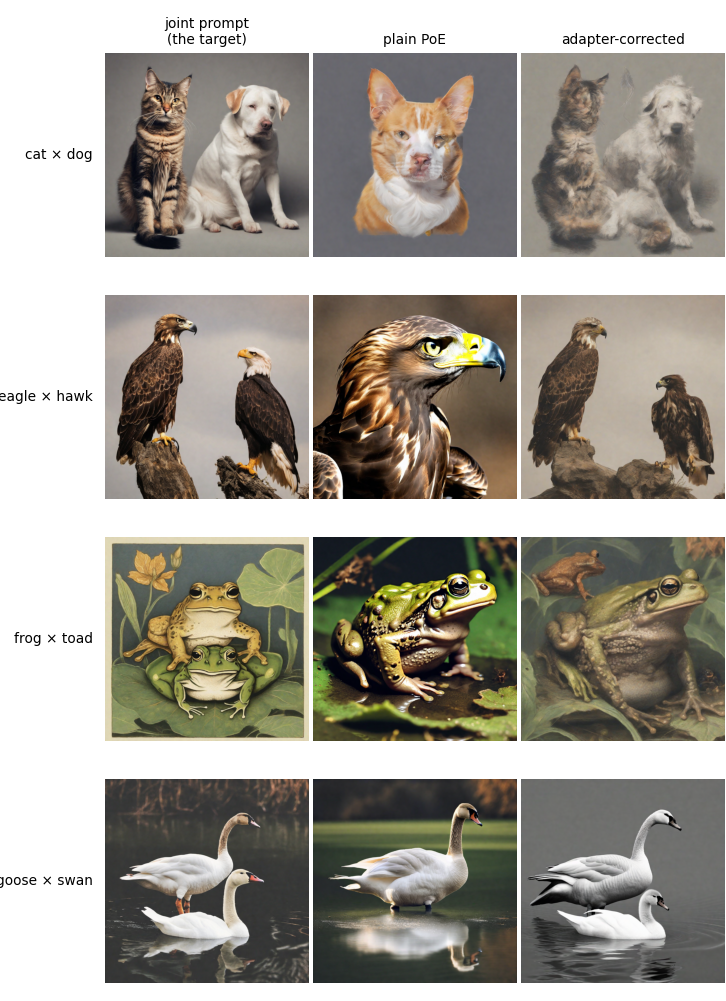
\includegraphics[width=\linewidth]{joint-prompt-poe-and-adapter-samples-for-four-held-out-pairs.pdf}
    \caption{\looseness=-1\textbf{The adapter returns held-out pairs to two animals without ever seeing the joint prompt.} Samples for four animal pairs held out of the adapter's training, under the joint prompt (left), plain product-of-experts composition (middle, one blended animal per row), and the adapter-corrected sampler (right, two distinct animals per row). The three images of a row start from the same noise, and the adapter column is the pooled checkpoint at training step 100000 with $\lambda=1$. The joint-prompt column is the target the correction was defined from, not a competing method. Four pairs illustrate the effect and do not carry the rate.}
    \label{fig:adapter-samples}
\end{wrapfigure}

A correction measured from the joint prompt is not a fix, because the joint prompt is exactly what composition is denied. The adapter removes that requirement. It is trained once on residuals cached from a pool of pairs, and at inference it produces the correction from the two concept prompts and the current state alone. The base model is frozen throughout, so what a domain has to hold is one small set of low-rank matrices rather than a retrained model. Pairs outside the training pool are corrected too, so what the adapter holds is not a stored correction per pair but the rule that restores plurality to a product of two experts. This matters most where joint data does not exist, since the residuals cached on the pairs that can be measured are enough to correct the pairs that cannot.

Training the adapter is not stable. Past a point the held-out renders stop moving toward the joint-prompt image and start losing colour and detail, while the adapter's weights keep growing and the loss stays flat. The pairs it trained on never show this, so what decays is the generalisation we actually want, and there is no signal in the training loss that says when to stop. Part of the cause is in how the correction was collected. Every state the adapter learns from lies on an uncorrected run, but a corrected run leaves that trajectory at its first corrected step, so at inference the adapter is asked for a correction at states it never saw. That error enters the next step, and the run moves further from anything in its training data as it goes. The adapter also inherits what sits beneath it, since it corrects a product of two frozen experts and neither the failures of a single expert nor the failures of the product are its to fix. It supplies the missing plurality term and nothing else, which is why corrected renders still carry the ordinary mistakes of the model underneath.

How much correction is needed, and when it has to arrive, are things we can measure but cannot predict. A composed run settles on one outcome or the other early, and the size of the correction at that moment says nothing about whether adding it will carry the run to the other side. We also have no way to follow the correction's direction across a run. It points somewhere different at every step, and the same pair started from different noise gives a different sequence of directions, so there is no single path to follow and no rule for which direction belongs at which step. Everything we know about how much to add, and when, came from sweeping those choices and reading the result. That is enough for a correction that works and not enough for one that can be steered.

What the paper leaves is a correction we can produce but not yet control. Two directions would change that. The first is the sampler. The correction is delivered during a run it was never computed for, and a sampler built to carry the correction while it runs would remove that mismatch rather than tolerate it. The second is the term itself. We studied one relation, two animals that both have to be present, and there is no reason the missing term takes the same form when the concepts are an object and its attribute, or an object and a place, or two things that cannot occupy the same region. Sorting the interaction term by the relation its concepts stand in, and by what goes missing in each case, is what would let composition be attempted in the wild rather than on a curated pool of pairs. Neither direction asks for a larger model.

\section{Conclusion}
\label{sec:conclusion}

Composing pretrained diffusion models as a product of experts assumes the concepts being composed are independent. When they are not, the product drops a term, and in the case we study that term is what makes both concepts appear at once instead of one blended thing. The term can be measured, adding it back causes composition, and a low-rank adapter can learn to produce it from the two concept prompts alone and supply it for pairs it never trained on. That changes what a composed model needs in practice. The concept pairs anyone actually wants rarely come with joint training data, and the correction learned on the pairs that can be measured carries to the ones that cannot. It also points at where capability might come from. If what is missing when two specialised models are composed is a term that can be learned once and reused, a set of small models with a learned correction between them is worth weighing against a single larger model trained to do everything, and that comparison is the experiment we would most like to see run.
% \section*{Ethics Statement}

% Lorem ipsum dolor sit amet, consectetur adipiscing elit. Integer tincidunt. Cras dapibus; vivamus elementum semper nisi. This placeholder should eventually discuss possible misuse, sensitive data, evaluation harms, environmental cost, or deployment constraints.

% \section*{Reproducibility Statement}

% Lorem ipsum dolor sit amet, consectetur adipiscing elit. Praesent congue erat at massa. Sed cursus turpis vitae tortor. This placeholder should eventually list code release status, random seeds, hardware, dataset provenance, hyperparameters, and any withheld artifacts.

% \section*{Acknowledgments}

% This anonymous placeholder contains no acknowledgments for submission. Replace this paragraph or remove the section for the initial blind review version if needed.

\bibliography{iclr2027_conference}
\bibliographystyle{iclr2027_conference}

% \appendix

% \section{Extended Related Work}
% \label{app:related}

% \subsection{Additional adaptation literature}

% Lorem ipsum dolor sit amet, consectetuer adipiscing elit. Aenean commodo ligula eget dolor. Aenean massa. Donec quam felis, ultricies nec, pellentesque eu, pretium quis, sem. This appendix slot is for adjacent methods that matter but would slow the main narrative.

% \subsection{Additional benchmarking literature}

% Nulla consequat massa quis enim. Donec pede justo, fringilla vel, aliquet nec, vulputate eget, arcu. In enim justo, rhoncus ut, imperdiet a, venenatis vitae, justo. This paragraph can become a longer comparison of benchmarks, threat models, and evaluation protocols.

% \subsection{Additional generation or exploration literature}

% Nullam dictum felis eu pede mollis pretium. Integer tincidunt. Cras dapibus; vivamus elementum semper nisi. Aenean vulputate eleifend tellus. This paragraph can become a longer bridge to diffusion models, search procedures, exploration policies, or sample generators.

% \section{Additional Method Details}
% \label{app:method-details}

% \subsection{Derivation of the product form and the plurality factor}
% \label{app:poe-derivation}

% Product-of-experts composition is obtained as follows \citep{liu2022compositional}.

% \begin{align}
% p(x \mid c_1, c_2)
%   &\propto p(x)\, p(c_1 \mid x)\, p(c_2 \mid x) \label{eq:independence}\\
%   &= p(x) \cdot \frac{p(x \mid c_1)\, p(c_1)}{p(x)} \cdot \frac{p(x \mid c_2)\, p(c_2)}{p(x)} \\
%   &= p(c_1)\, p(c_2) \cdot \frac{p(x \mid c_1)\, p(x \mid c_2)}{p(x)} \\
%   &\propto \frac{p(x \mid c_1)\, p(x \mid c_2)}{p(x)}
% \end{align}

% The unconditional density is in the denominator because it is already contained in both conditional experts, so their product carries it twice and one copy has to be removed.

% The gap between the joint conditional and the product form can be written as

% \begin{align}
% R_t &\;\equiv\; \frac{p(c_1, c_2 \mid x_t)}{p(c_1 \mid x_t)\, p(c_2 \mid x_t)}\\
% p(c_1, c_2 \mid x_t) &= p(c_1 \mid x_t)\, p(c_2 \mid x_t)\, R_t
% \end{align}

% $R_t$ equals one exactly when the two concepts are independent given the state. Carrying it through the same Bayes steps recovers the joint conditional from the product form.

% \begin{align}
% p(x_t \mid c_1, c_2)
%   &\propto p(x_t)\, p(c_1, c_2 \mid x_t) \\
%   &= p(x_t)\, p(c_1 \mid x_t)\, p(c_2 \mid x_t)\, R_t \\
%   &\propto p(x_t)\, \frac{p(x_t \mid c_1)}{p(x_t)}\, \frac{p(x_t \mid c_2)}{p(x_t)}\, R_t
%   &&\text{(Bayes on each factor, as in \eqref{eq:independence})}\\
%   &\propto \frac{p(x_t \mid c_1)\, p(x_t \mid c_2)}{p(x_t)}\, R_t \\
%   &\propto p_{\mathrm{PoE}}(x_t \mid c_1, c_2)\, R_t
% \end{align}

% Taking the gradient of the logarithm of both sides, and converting scores to noise predictions, gives the relation between the true joint prediction and the product-of-experts prediction stated in Section~\ref{sec:interaction}.

% \subsection{Derivation of the placeholder objective}

% Lorem ipsum dolor sit amet, consectetur adipiscing elit. Let $\theta^{\star}$ denote the best adapted parameter under the placeholder score:
% \begin{equation}
%     \theta^{\star}
%     =
%     \argmin_{\theta'}
%     \left[
%     \mathcal{L}(\theta')
%     +
%     \eta
%     \left\|
%     \nabla_{\theta'} \mathcal{L}(\theta')
%     \right\|_{2}^{2}
%     \right].
%     \label{eq:appendix-objective}
% \end{equation}
% Sed ut perspiciatis unde omnis iste natus error sit voluptatem accusantium doloremque laudantium. Replace this derivation with the real loss, estimator, theorem, or convergence argument.

% \subsection{Placeholder proposition}

% \newtheorem{proposition}{Proposition}
% \begin{proposition}[Placeholder stability]
% Assume the score in Eq.~\ref{eq:score} is $L$-Lipschitz in $\theta'$ and that the adaptation operator in Eq.~\ref{eq:adaptation} changes by at most $\epsilon$ under a single-regime perturbation. Then the reported score changes by at most $L\epsilon$.
% \end{proposition}

% \paragraph{Proof sketch.}
% Lorem ipsum dolor sit amet, consectetur adipiscing elit. By the Lipschitz assumption,
% \begin{equation}
%     \left|S(\theta'_{a},\mathcal{D}_{2}) - S(\theta'_{b},\mathcal{D}_{2})\right|
%     \leq
%     L\left\|\theta'_{a}-\theta'_{b}\right\|_{2}
%     \leq
%     L\epsilon.
% \end{equation}
% Quisque rutrum aenean imperdiet. Etiam ultricies nisi vel augue. Replace this proof sketch with the real theorem or delete it if the paper is purely empirical.

% \subsection{Implementation notes}

% Suspendisse potenti. Sed lectus. Integer euismod lacus luctus magna. Quisque cursus, metus vitae pharetra auctor, sem massa mattis sem, at interdum magna augue eget diam. Use this subsection for architecture details, preprocessing choices, batching, optimizer settings, and implementation deviations from prior work.

% \section{Additional Experimental Results}
% \label{app:additional-results}

% \subsection{Full metric matrix}

% Lorem ipsum dolor sit amet, consectetur adipiscing elit. Phasellus viverra nulla ut metus varius laoreet. Table~\ref{tab:full-matrix} is a fake expanded result table for all regimes and metrics.

% \begin{table}[h]
% \caption{Placeholder full metric matrix}
% \label{tab:full-matrix}
% \begin{center}
% \begin{tabular}{lcccccc}
% \hline
% \textbf{Method} & \textbf{U1} & \textbf{U2} & \textbf{R1} & \textbf{R2} & \textbf{C1} & \textbf{C2} \\
% \hline
% Baseline A & 71.2 & 68.9 & 22.4 & 19.5 & 1.00 & 0.82 \\
% Baseline B & 73.5 & 69.4 & 20.1 & 18.7 & 1.18 & 0.79 \\
% \methodname & 78.9 & 75.6 & 16.3 & 14.2 & 1.09 & 0.76 \\
% Oracle & 82.0 & 78.2 & 12.0 & 10.5 & 2.40 & 0.64 \\
% \hline
% \end{tabular}
% \end{center}
% \end{table}

% \subsection{Additional curves}

% Morbi nec metus. Phasellus blandit leo ut odio. Maecenas ullamcorper, dui et placerat feugiat, eros pede varius nisi, condimentum viverra felis nunc et lorem. Figure~\ref{fig:appendix-curves} is reserved for secondary sweeps or per-domain curves.

% \begin{figure}[h]
% \placeholderfigure{1.75in}{Appendix curves}
% \caption{Placeholder appendix curves. Replace with per-domain plots, seed-level traces, or confidence intervals.}
% \label{fig:appendix-curves}
% \end{figure}

% \subsection{Qualitative examples}

% Donec vitae sapien ut libero venenatis faucibus. Nullam quis ante. Etiam sit amet orci eget eros faucibus tincidunt. This subsection can hold generated samples, rollouts, extracted examples, failure cases, or visual inspection panels.

% \begin{figure}[h]
% \placeholderfigure{1.85in}{Qualitative examples}
% \caption{Placeholder qualitative examples. Replace with representative successes and failures, not only favorable cases.}
% \label{fig:qualitative}
% \end{figure}

% \section{Experimental Details}
% \label{app:experimental-details}

% \subsection{Datasets, domains, and splits}

% Lorem ipsum dolor sit amet, consectetur adipiscing elit. Vestibulum ullamcorper mauris at ligula. Fusce fermentum odio nec arcu. Table~\ref{tab:hyperparameters} is a placeholder for reproducibility-critical settings.

% \begin{table}[h]
% \caption{Placeholder hyperparameters}
% \label{tab:hyperparameters}
% \begin{center}
% \begin{tabular}{ll}
% \hline
% \textbf{Setting} & \textbf{Value} \\
% \hline
% Batch size & 128 \\
% Learning rate & $3 \times 10^{-4}$ \\
% Training steps & 100,000 \\
% Evaluation seeds & 10 \\
% Selection metric & Validation score \\
% Hardware & Placeholder accelerator \\
% \hline
% \end{tabular}
% \end{center}
% \end{table}

% \subsection{Baselines and implementations}

% Pellentesque auctor neque nec urna. Proin sapien ipsum, porta a, auctor quis, euismod ut, mi. Aenean viverra rhoncus pede. Replace this with exact baseline names, official repositories, commit hashes, and any local modifications.

% \subsection{Compute resources}

% Vivamus elementum semper nisi. Aenean vulputate eleifend tellus. Aenean leo ligula, porttitor eu, consequat vitae, eleifend ac, enim. Replace this with accelerator type, wall-clock cost, memory footprint, and total experiment budget.

% \section{Limitations, Broader Impact, and LLM Use}
% \label{app:limitations}

% \subsection{Limitations}

% Lorem ipsum dolor sit amet, consectetur adipiscing elit. Suspendisse enim turpis, dictum sed, iaculis a, condimentum nec, nisi. Praesent nec nisl a purus blandit viverra. Replace this with the strongest known caveats, including assumptions that future reviewers are likely to probe.

% \subsection{Broader impact}

% Nullam vel sem. Nam ipsum risus, rutrum vitae, vestibulum eu, molestie vel, lacus. Sed magna purus, fermentum eu, tincidunt eu, varius ut, felis. Replace this with a domain-specific risk and benefit analysis.

% \subsection{Use of large language models}

% In the preparation of this placeholder manuscript, language models may be used for drafting filler, refactoring prose, and checking consistency. Replace this statement with the final, accurate disclosure for the submitted paper.

\end{document}
